\documentclass[a4paper]{report}

\usepackage[T2A]{fontenc}
\usepackage[english,russian]{babel}
\usepackage{amsmath}
\usepackage{amssymb}
\usepackage{paracol}
\usepackage[14pt]{extsizes}
\usepackage[left=30mm, top=20mm, right=15mm, bottom=20mm, footskip=15mm]{geometry}
\usepackage[style=gost-numeric,sorting=none]{biblatex}
\usepackage{graphicx}
\usepackage[hidelinks]{hyperref}
\usepackage{minted}
\usepackage{caption}
\usepackage{tabularx}
\usepackage{changepage}
\usepackage{titlesec}
\usepackage{lipsum}
\usepackage[normalem]{ulem}
\usepackage{indentfirst}
\usepackage{ragged2e}
\usepackage{longtable}
\usepackage{setspace}
\usepackage{url}

\setlength\parindent{1.25cm}

\titleformat{\chapter}[hang]
  {\normalfont\LARGE\bfseries}{\thechapter}{1em}{}

\setminted{fontsize=\footnotesize}
\setminted{breaklines=true}

\captionsetup[listing]{name=Листинг}

\addbibresource{sources.bib}

\graphicspath{ {./assets/} }

% Planner Component
% these are important parts of the planner
\newcommand{\pc}[1]{\textit{#1}}
% CoDe element
% these are the specific structs or traits
% and so on in the program
\newcommand{\cd}[1]{\texttt{#1}}
% JARgon
% and other important things,
% like pattern names
\newcommand{\jar}[1]{\textit{#1}}

\hyphenpenalty=2000
\exhyphenpenalty=5000

\begin{document}

\newgeometry{left=30mm, top=1mm, right=20mm, bottom=1mm}

\setstretch{1}

\begin{titlepage}

  \begin{center}
    \hfill \break
    \small
    \textbf{
      МИНИСТЕРСТВО НАУКИ И ВЫСШЕГО ОБРАЗОВАНИЯ\\
      РОССИЙСКОЙ ФЕДЕРАЦИИ\\
      ФЕДЕРАЛЬНОЕ ГОСУДАРСТВЕННОЕ АВТОНОМНОЕ ОБРАЗОВАТЕЛЬНОЕ\\
      УЧРЕЖДЕНИЕ ВЫСШЕГО ОБРАЗОВАНИЯ\\
      <<РОССИЙСКИЙ УНИВЕРСИТЕТ ДРУЖБЫ НАРОДОВ\\
      ИМЕНИ ПАТРИСА ЛУМУМБЫ>>
    }\\
    \normalsize
    Факультет \underline{физико-математических и естественных наук}\\ 
    Кафедра \underline{математического моделирования и искусственного интеллекта}

    \vspace*{\fill}

    \begin{flushright}
      <<Допустить к защите>>\\
      Заведующий кафедрой\\
      математического моделирования\\и искусственного интеллекта\\
      д.ф-м.н., доцент\\
      \underline{\phantom{signature signa}} Малых М.Д.\\
      <<\underline{\phantom{day}}>> \underline{\phantom{month month}} 2025 г.
    \end{flushright}
   
    \vspace*{\fill}
    \Large{\textbf{Выпускная квалификационная работа\\ бакалавра}}
    \\
    \normalsize
    Направление  09.03.03 <<\underline{Прикладная информатика}>>
  \end{center}

  \vspace*{\fill}

  \begin{justify}
    \mbox{ТЕМА \uline{<<Мультиагентное планирование в условиях несогласованности целей>>}} \\
    Выполнил студент \underline{\textbf{Матюхин Григорий Васильевич}}
  \end{justify}

  \vspace*{\fill}

  \noindent \begin{tabular}{p{0.5\linewidth} c}
      Группа \underline{НПИбд-01-21} & Руководитель выпускной  \\
      & квалификационной работы\\
      Студ. билет \textnumero{} \underline{1032211403} & \underline{Виноградов Андрей Николаевич,}\\
      & \underline{к.ф.-м.н., доцент кафедры ММиИИ} \\
      \\
      & \underline{\phantom{signature signature signature sig}} \\
      \\
      \\
      & Автор \underline{\phantom{signature signature signat}} \\
    \end{tabular}
   \vspace*{\fill}
   
  \begin{center} \textbf{г. Москва} \\ 2025 г. \end{center}
  \thispagestyle{empty} % выключаем отображение номера для этой страницы
   
\end{titlepage}

\restoregeometry

\setstretch{1.2}
\begin{center}
  \textbf{Федеральное государственное автономное образовательное учреждение высшего образования} \\
  \textbf{<<Российский университет дружбы народов}\\
  \textbf{имени Патриса Лумумбы>>}\\

  \large \textbf{АННОТАЦИЯ}\\
  \normalsize \textbf{выпускной квалификационной работы} \\

  \underline{Матюхина Григория Васильевича}
\end{center}

на тему: \uline{Мультиагентное планирование в условиях несогласованности целей}

В данной работе рассматривается проблема мультиагентного планирования
в условиях несогласованности целей между агентами.
Основное внимание уделяется разработке и реализации планировщика,
способного координировать действия автономных агентов,
обладающих индивидуальными наборами целей
и функционирующих в общем пространстве состояний.
В работе проведён систематический обзор
существующих методов разрешения конфликтов и кооперации
в мультиагентных системах с использованием методологии PRISMA-ScR,
что позволило выявить ограничения текущих подходов
и сформулировать требования к архитектуре собственной системы.
Разработанный планировщик реализован на языке Rust
и способен функционировать на встраиваемых устройствах.
Его архитектура включает поддержку эвристического анализа достижимости целей,
механизмов приоритезации, обмена планами и устойчивого поведения
в условиях частичной недостижимости целей.
Результаты демонстрируют применимость предложенного решения в распределённых сценариях,
таких как рои роботов и логистические сети,
что подтверждает актуальность и практическую значимость работы.

\vspace*{\fill}

\noindent \begin{tabular}{p{0.33\linewidth} p{0.33\linewidth} p{0.33\linewidth}}
Автор ВКР & \underline{\phantom{signature sign}} & \underline{\phantom{Матюхин Григорий}} \\
& (Подпись) & (ФИО)
\end{tabular}

\thispagestyle{empty} 


\setstretch{1.5}

\setcounter{page}{3}  

\tableofcontents

\chapter*{Введение}
\addcontentsline{toc}{chapter}{Введение}

\section*{Актуальность работы}

С ростом сложности распределённых систем и увеличением числа взаимодействующих
интеллектуальных компонентов возникает потребность
в эффективных методах планирования и координации действий.
Мультиагентные системы находят широкое применение в таких сферах,
как логистика, управление беспилотными устройствами,
моделирование и робототехника.
Однако одной из ключевых проблем остаётся разрешение противоречий между целями агентов,
действующих в общем пространстве. 
Существующие решения либо ориентированы на строго кооперативные сценарии,
либо не масштабируются при увеличении числа агентов.
Это обуславливает необходимость разработки архитектур и алгоритмов,
способных учитывать несовпадающие цели,
обеспечивать частичную автономию агентов и устойчивость системы
при частичной недостижимости целей.
Настоящая работа направлена на создание планировщика, способного решать подобные задачи.

\section*{Цели работы}

Целью работы является разработка архитектуры
и программной реализации планировщика,
обеспечивающего согласование действий агентов
в мультиагентной системе при наличии потенциально конфликтующих целей.

\section*{Задачи работы}

Для достижения поставленной цели необходимо решить следующие задачи:
\begin{itemize}
  \item Провести обзор современных методов планирования и кооперации в мультиагентных системах;
  \item Проанализировать подходы к разрешению конфликтов между агентами;
  \item Разработать и реализовать одноагентный планировщик как основу для мультиагентного решения;
  \item Спроектировать мультиагентную архитектуру,
    обеспечивающую взаимодействие агентов, оценку достижимости целей и обмен планами;
  \item Реализовать методы устойчивого планирования с учётом частичной недостижимости целей;
  \item Оценить корректность и применимость разработанного подхода на демонстрационных сценариях.
\end{itemize}

\section*{Апробация работы}

В ходе выполнения работы были получены результаты, представленные на
Всероссийской конференции с международным участием
<<Информационно"=телекоммуникационные технологии
и математическое моделирование высокотехнологичных систем>> (Москва, РУДН, 2025 г.).

\section*{Публикации}

По теме выпускной квалификационной работы бакалавра была опубликована работа~\cite{ittmm}.

\section*{Структура работы}

Работа состоит из введения, трех глав, заключения и списка литературы.
Во введении отражена проблематика выбранной
темы, актуальность этой темы в современном мире,
поставлены цели и задачи данной работы.
Первая глава посвящена систематическому обзору существующих методов планирования, кооперации и разрешения конфликтов в мультиагентных системах. Третья глава описывает реализацию одноагентного планировщика: архитектуру, внутренние структуры и принципы работы. В четвёртой главе рассматривается переход к мультиагентной системе: уточнение целей, межагентная коммуникация и устойчивость. Заключение содержит основные выводы и направления дальнейших исследований.

\section*{Справочная информация}

\subsection*{Мультиагентные системы}

Мультиагентные системы (MAS, \textit{Multi-Agent System}) играют центральную роль в искусственном интеллекте,
обеспечивая децентрализованное принятие решений в таких областях, как автономные
транспортные средства, интеллектуальные энергосистемы и робототехника~\cite{Torre_o_2017}.
Их масштабируемость, адаптивность и отказоустойчивость делают их незаменимыми
для сложных, динамических сред, требующих кооперации и разрешения конфликтов.

Несмотря на достижения, остаются проблемы, связанные с эффективной координацией
и разрешением конфликтов~\cite{galesloot2024factoredonlineplanningmanyagent}
\cite{zhang2014formalanalysisrequiredcooperation}. Такие методы, как задачи удовлетворения
ограничений (CSP, \textit{Constraint Satisfaction Problem})~\cite{KOMENDA201476} и модели, основанные на переговорах
\cite{GROSZ1996269,RABELO1994303}, демонстрируют потенциал, но часто сталкиваются
с проблемами масштабируемости в реальных условиях. Кроме того, отсутствие единых
оценочных метрик затрудняет сравнительный анализ.


\subsection*{Планирование}

Планирование в области искусственного интеллекта представляет собой процесс автоматического построения последовательности действий, необходимых для достижения цели. Классическое планирование предполагает полное знание среды, детерминированность действий и статичность мира. Однако в реальных приложениях — особенно в мультиагентных системах — нередко возникают ситуации с неполной информацией, конкурирующими интересами и необходимостью адаптации плана в процессе выполнения. Это требует разработки более гибких моделей, способных учитывать множественность целей и агентов, действующих независимо.

\subsection*{Планировщики}

Планировщики~\cite{ghallab2004automated} --- это системы, используемые для автоматического создания последовательности действий, необходимых для достижения заданной цели в определенной среде. Они широко применяются в различных областях, таких как робототехника, логистика, искусственный интеллект и управление задачами. Основная задача планировщика заключается в нахождении оптимального или приемлемого плана, который переводит систему из начального состояния в целевое состояние, удовлетворяя при этом заданным ограничениям и условиям.

\subsection*{Planning Domain Definition Language}

PDDL (Planning Domain Definition Language)~\cite{mcdermott1998pddl}~\cite{gerevini2006pddl3}
--- это язык описания задач планирования, используемый в области искусственного интеллекта.
Он позволяет формализовать модель мира и определить цели, которых необходимо достичь.
Обычно описание задачи в PDDL состоит из двух основных файлов:
\textit{файла домена} и \textit{файла задачи}.
Это деление позволяет отделить общую модель мира (правила, действия, объекты и свойства)
от конкретной задачи, которая решается в рамках этого мира.

\begin{enumerate}
\item \textbf{Файл домена} описывает, какие действия возможны в рассматриваемом мире,
  какие предикаты используются для описания состояния,
    и как действия изменяют это состояние.
    Ниже приведён пример PDDL-домена для маленького склада:

  \begin{minted}{lisp}
(define (domain mini-warehouse)
  (:requirements :strips :typing :quantified-preconditions)
  (:types robot box location)
  (:predicates
    (at ?r - robot ?l - location)
    (box-at ?b - box ?l - location)
    (carrying ?r - robot ?b - box)
    (clean ?l - location)
    (adjacent ?l1 - location ?l2 - location) )
  (:action move
    :parameters (?r - robot ?from - location ?to - location)
    :precondition (and (at ?r ?from) (adjacent ?from ?to))
    :effect (and (not (at ?r ?from)) (at ?r ?to)) )
  (:action pick-up
    :parameters (?r - robot ?b - box ?l - location)
    :precondition (and (at ?r ?l) (box-at ?b ?l))
    :effect (and (carrying ?r ?b) (not (box-at ?b ?l))) )
  (:action drop
    :parameters (?r - robot ?b - box ?l - location)
    :precondition (and (at ?r ?l) (carrying ?r ?b))
    :effect (and (box-at ?b ?l) (not (carrying ?r ?b))) )
  (:action clean-nearby
    :parameters (?r - robot ?l - location)
    :precondition (at ?r ?l)
    :effect (forall (?x - location)
      (when (adjacent ?l ?x) (clean ?x))))
)
  \end{minted}

    В этом примере моделируется поведение роботов на складе:
    перемещение между локациями, управление коробками и очистка территорий.
    Используются возможности языка PDDL:
    \begin{itemize}
      \item \texttt{:strips},
      \item \texttt{:typing},
      \item \texttt{:quantified-preconditions}.
    \end{itemize}
    Определены три типа объектов: роботы, коробки, локации.
    Предикаты задают положение роботов и коробок, факт переноски, чистоту и смежность локаций.
    Действия позволяют роботу: перемещается между соседними локациями,
    поднимать коробку из текущей локации, опускать коробку в текущей локации, очищать все смежные с текущей локации.

\item \textbf{Файл задачи} указывает,
  какие объекты существуют в данной конкретной задаче,
    каково начальное состояние и какое целевое состояние требуется достичь.
    Вот пример соответствующего файла задачи:

  \begin{minted}{lisp}
(define (problem mini-a)
  (:domain mini-warehouse)
  (:objects
    r1 - robot
    b1 b2 - box
    l1 l2 l3 - location)
  (:init
    (at r1 l1)
    (box-at b1 l2)
    (box-at b2 l3)
    (adjacent l1 l2)
    (adjacent l2 l3)
    (adjacent l1 l3))
  (:goal (and
    (box-at b1 l3)
    (clean l2)))
)
  \end{minted}

  Здесь задача использует домен \texttt{mini-warehouse}. 
  В задаче заданы: один робот, две коробки, три локации.
  Робот находится в \texttt{l1}, коробки \texttt{b1} и \texttt{b2} -- в \texttt{l2} и \texttt{l3} соответственно.
  Все локации попарно смежны.
  Целью является: коробка \texttt{b1} находится в локации \texttt{l3} и локация \texttt{l2} должна быть очищена.
\end{enumerate}

Такое разделение обеспечивает переиспользуемость:
один и тот же домен можно использовать для множества различных задач.
Кроме того, это упрощает тестирование и отладку планирующих систем.
Благодаря своей формальной структуре PDDL поддерживает автоматическую проверку корректности задач
и их совместимости с определением домена,
что делает его мощным инструментом для разработки и исследования алгоритмов планирования.

Решением для такой этой конкретной проблемы будет следующая последовательность действий:
\begin{minted}{lisp}
(
  (move r1 l1 l2)
  (pick-up r1 b1 l2)
  (move r1 l2 l3)
  (drop r1 b1 l3)
  (clean-nearby r1 l3)
)
\end{minted}

Задача планировщика --- принять на вход описание домена и задачи, и вывести последовательность действий для ее решения.

\chapter{Анализ существующих методик}

В этом обзоре систематически анализируются методологии и исследовательские пробелы
с использованием PRISMA-ScR~\cite{prisma-src}, с акцентом на моделирование предметной
области, разрешение конфликтов и механизмы кооперации. Цель --- предоставить основу
для будущих разработок MAS, способствующих их более широкому применению в реальных
сценариях.

Ключевые цели исследования:

\begin{enumerate}
  \item Определение распространенных подходов к моделированию MAS.
  \item Анализ стратегий разрешения конфликтов.
  \item Исследование механизмов кооперации.
  \item Оценка эффективности существующих методологий.
\end{enumerate}

\section{Методы} 

\subsection{Протокол и регистрация}

Настоящий обзор следует структуре PRISMA-ScR~\cite{prisma-src},
обеспечивая систематичность и прозрачность изложения.
Перед сбором данных были определены исследовательские цели,
критерии включения и стратегии поиска.
Протокол не был зарегистрирован в PROSPERO,
так как скопинговые обзоры не входят в его сферу.\footnote{С протоколом можно ознакомится по ссылке 
\url{https://gmatiukhin.site/articles/MAS-Conflict-Solving-Review/}}

\subsection{Критерии отбора}

Данный обзор основан на структуре \jar{Популяция, Концепция, Контекст}
(Population, Concept, Context, PCC)~\cite{afc61c6cf471416489e36a4bc382d3b9}.
В него включены исследования, посвященные методам кооперации в системах с несколькими автономными агентами.
Под <<автономным агентом>> понимается интеллектуальный объект,
способный воспринимать окружающую среду,
принимать решения и действовать самостоятельно в рамках вычислительных и коммуникационных ограничений.
Это определение не ограничивается только роботами или беспилотными транспортными средствами.
Обзор включает как качественные, 
так и количественные эмпирические исследования,
исключая комментарии, аналитические заметки и тезисы конференций.

\begin{table}
  \centering
  \begin{footnotesize}
  \caption{Критерии включения/исключения}
  \label{tab:criteria}
  \begin{longtable}{|p{0.15\textwidth}|p{0.2\textwidth}|p{0.2\textwidth}|p{0.35\textwidth}|}
    \hline
    Критерий & Включение & Исключение & Обоснование\\
    \hline
    \hline
 Популяция        & Системы с несколькими автономными агентами, работающими как в реальных (роевые роботы, системы доставки), так и в виртуальных или симулированных средах. & Системы с одним агентом.                                                              & В обзоре рассматриваются кооперация и разрешение конфликтов, что неактуально для систем с одним агентом.                  \\
    \hline
 Концепция        & Алгоритмы, обеспечивающие кооперацию между автономными агентами в MAS.                                                                                   & Алгоритмы, ориентированные только на одиночные агенты.                                & Обзор сосредоточен на алгоритмах, способствующих кооперации в MAS.                                                        \\
    \hline
 Контекст         & Исследования, посвященные разработке алгоритмов кооперативного планирования и разрешения конфликтов в MAS с элементами искусственного интеллекта.        & Исследования, касающиеся разрешения конфликтов вне области искусственного интеллекта. & Обзор ориентирован исключительно на алгоритмы в области искусственного интеллекта, остальные области не рассматриваются.  \\
    \hline
 Язык             & Английский, русский, немецкий.                                                                                                                           & Другие языки.                                                                         & Рецензенты владеют только английским, русским и немецким языками и не имеют ресурсов для перевода статей с других языков. \\
    \hline
 Типы источников  & Рецензируемые научные статьи, эмпирические исследования.                                                                                                 & Нерецензируемые статьи, комментарии, письма в редакцию.                               & Использование рецензируемых источников гарантирует надежность и научную обоснованность представленных данных.             \\
    \hline
 Географический   & Любые страны.                                                                                                                                            & Нет исключений.                                                                       & Исследование кооперации и разрешения конфликтов в MAS не зависит от страны происхождения.                                 \\
    \hline
 Временной период & Любой.                                                                                                                                                   & Нет исключений.                                                                       & Область исследования достаточно узкая, поэтому решено включить все доступные научные работы.                              \\
    \hline
  \end{longtable}
  \end{footnotesize}
\end{table}

\subsection{Источники информации}

Поиск литературы проводился преимущественно в ScienceDirect,
выбранном из-за его обширного репозитория рецензируемых статей
по разрешению конфликтов и кооперации в MAS.
Дополнительно проводился поиск по цитированиям для выявления
важных исследований, которые могли быть пропущены. Списки литературы
включенных исследований были вручную проверены на наличие других
потенциально релевантных источников.

\subsection{Стратегия поиска}

\begin{table}[h!]
  \centering
  \begin{footnotesize}
  \caption{Извлекаемая информация}
  \label{tab:questions}
  \renewcommand{\arraystretch}{1.3}
  \begin{tabular}{|p{5cm}|p{9cm}|}
    \hline
    \multicolumn{2}{|c|}{\textbf{Сведения о публикации}} \\
    \hline
    Название исследования & - \\
    \hline
    Автор(ы) & Кто автор(ы) исследования/документа? \\
    \hline
    Год публикации & В каком году было опубликовано исследование? \\
    \hline
    Тип публикации & Является ли документ эмпирическим исследованием? \\
    \hline
    Страна происхождения & В какой стране было выполнено исследование? \\
    \hline

    \multicolumn{2}{|c|}{\textbf{Общие сведения}} \\
    \hline
    Цели/назначение & Каковы цели исследования/документа? \\
    \hline
    Дизайн исследования & Каков дизайн исследования/документа? \\
    \hline
    Контекст исследования & Какую реальную или воображаемую систему описывает исследование? \\
    \hline
    Популяция & Как описывается многоагентная система? \\
    \hline

    \multicolumn{2}{|c|}{\textbf{Содержательная часть}} \\
    \hline
    Методология & Какова предметная область? \\
    \cline{2-2}
     & Как моделируется предметная область? \\
    \cline{2-2}
     & Описание алгоритма \\
    \cline{2-2}
     & Является ли алгоритм специфичным для области? \\
    \hline
    Оценка результатов & Как определяется «успех»? \\
    \cline{2-2}
     & Как оценивается алгоритм? \\
    \cline{2-2}
     & Каковы преимущества алгоритма? \\
    \hline
    \end{tabular}
  \end{footnotesize}
\end{table}

Стратегия поиска была тщательно разработана с целью систематического выявления
научных публикаций, посвящённых вопросам кооперации в MAS.
Изначально был проведён разведочный поиск для выявления релевантной терминологии
и определения преобладающих исследовательских тем в данной области.
Этот этап имел решающее значение для точного выбора поисковых ключевых слов,
обеспечивая, чтобы последующие запросы были одновременно точными и исчерпывающими.
Для повышения эффективности поиска использовались продвинутые методы,
такие как булевы операторы и символы усечения.
Эти методы способствовали охвату широкого спектра лексических
вариаций и синонимичных терминов, тем самым расширяя рамки литературного обзора.
Использованные поисковые запросы:

\begin{itemize}
  \item \texttt{multi-agent systems AND conflict solving}
  \item \texttt{cooperated planning AND conflict solving}
  \item \texttt{multi-agent systems AND cooperated planning}
  \item \texttt{multi-agent systems AND (cooperated planning OR conflict solving)}
\end{itemize}

Итеративный характер поискового процесса позволял непрерывно уточнять стратегию,
адаптируясь к новой информации, выявленной в ходе обзора.
Помимо автоматизированных поисков в базах данных,
стратегия включала ручной анализ списков литературы в отобранных исследованиях.
Этот дополнительный подход сыграл ключевую роль в идентификации основополагающих работ
и дополнительных источников, которые могли быть упущены при исключительно электронном поиске.
Интеграция автоматических и ручных методов обеспечила всесторонний анализ
языковых нюансов, культурных особенностей и специфических вызовов в области MT.
В конечном итоге, данная комплексная стратегия поиска создала прочную основу для обзора,
обеспечив глубокое и многогранное понимание
различных методологий, направленных на обеспечение кооперации в MAS.
Подробное описание извлекаемой информации приведено в таблице~\ref{tab:questions}

\subsection{Выбор источников данных}

Заголовки и аннотации найденных статей просматривались одним рецензентом.
Если возникала неопределённость относительно включения статьи
на этапе первичного просмотра, она также включалась для полнотекстовой оценки.
Статьи, которые потенциально соответствовали
критериям включения/исключения (таблица~\ref{tab:criteria}),
переходили к этапу полнотекстового анализа.
Аналогично просмотру заголовков и аннотаций, статьи оценивались одним рецензентом.
Итоговые результаты поиска, включая количество просмотренных,
включённых и исключённых статей на каждом этапе,
были представлены в виде диаграммы потоков PRISMA (рис.~\ref{fig:PRISMA}),
в соответствии с рекомендациями PRISMA-ScR. Это визуально отображает
процесс отбора исследований и обеспечивает соответствие стандартам отчётности.

\subsection{Процесс извлечения данных}

Извлечение данных выполнялось одним членом исследовательской группы,
в соответствии с методологией JBI~\cite{afc61c6cf471416489e36a4bc382d3b9}.
Извлекаемые данные включали характеристики исследований и особенности
мультиагентных автономных систем, релевантные исследовательским вопросам\footnote{С промежуточными результатами можно ознакомится по ссылке
\url{https://gmatiukhin.site/articles/MAS-Conflict-Solving-Review/}}.

\subsection{Элементы данных}

\subsubsection{Синтез результатов}

\paragraph{Обобщение и суммирование результатов}

Первичный анализ включал как количественные, так и качественные методы.
Был проведен описательный числовой анализ исследований, охватывающий
количество работ, годы публикации, исследуемые популяции и ключевые методологии.
На основе исследовательских вопросов был проведен дедуктивный контент-анализ,
а также представлено нарративное описание табличных данных.

\paragraph{Представление результатов}

Результаты представлены в соответствии с рекомендациями PRISMA-ScR.
Диаграмма потока PRISMA (рис.~\ref{fig:PRISMA}) иллюстрирует процесс выбора исследований,
включая причины исключения на этапе полного текстового анализа.
Количественные результаты представлены в таблицах и сопровождаются
описательным анализом, согласующимся с исследовательскими вопросами.

\section{Результаты}

\subsection{Отбор источников данных}

В ходе поиска по базе ScienceDirect с использованием заданных поисковых запросов было выявлено 21770 исследований.
После удаления 4562 дубликатов (20,95\%) осталось 17203 уникальных записи.
Автоматизированные инструменты исключили 13371 исследование (82,37\%)
на основании их нерелевантности или недостаточной эмпирической/теоретической проработки вопросов,
связанных с мультиагентными системами, сотрудничеством и разрешением конфликтов.
Далее 3837 исследований (17,62\%) были отобраны для анализа на основе критериев включения/исключения.

На следующем этапе 76 публикаций (0,34\%) были отобраны для ручного анализа, из которых 75 были рассмотрены.
Из них 58 исследований (77,33\%) были исключены по следующим причинам:

\begin{itemize}
  \item 35 исследований (46,67\%) рассматривали исключительно теоретические основы;
  \item 12 исследований (16,00\%) не затрагивали ключевые аспекты сотрудничества в мультиагентных системах
    или их проектирования, включая моделирование домена или описание алгоритмов;
  \item 6 исследований (8,00\%) представляли собой систематические обзоры литературы без детализированных методологических аспектов;
  \item 5 исследований (6,67\%) были библиографическими обзорами и не содержали оригинальных эмпирических данных.
\end{itemize}

В результате в данный обзор было включено 17 исследований (0,07\% от общего числа записей).
Дополнительно с помощью поиска по цитированию были выявлены ещё 6 исследований, однако лишь 2 из них были включены в анализ.
В совокупности 19 исследований обеспечили релевантные эмпирические данные, теоретические основы,
а также представления о методах разрешения конфликтов и алгоритмах сотрудничества в мультиагентных системах,
включая терминологию, специфичную для данной области.

\begin{figure}
  \centering
  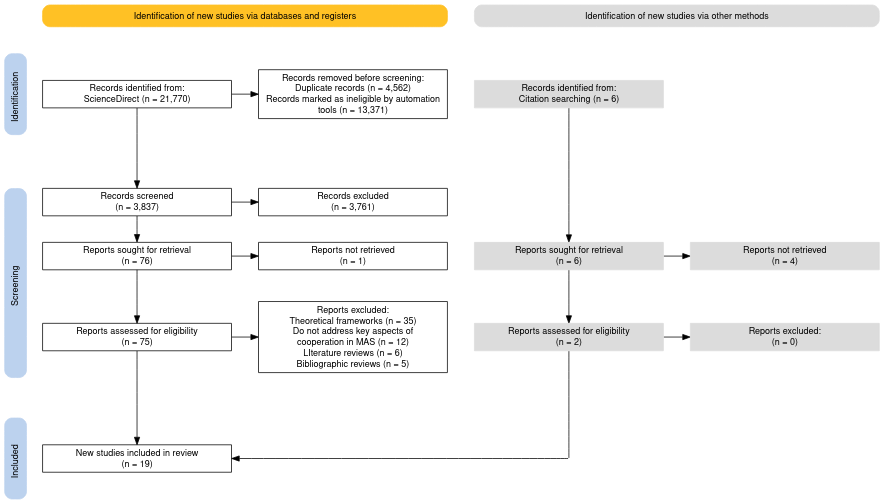
\includegraphics[width=0.8\linewidth]{PRISMA.png}
  \caption{PRISMA Flow Diagram}
  \label{fig:PRISMA}
\end{figure}

\subsubsection{Анализ временного распределения}

Анализ временной шкалы публикаций показывает стабильный, хотя и медленный,
темп появления новых статей в период с 1988 по 2001 год (рис.~\ref{fig:articles-by-year}).
Затем наблюдается десятилетний разрыв до 2011 года,
после которого количество публикаций удвоилось по сравнению с 1988-2001 годами.
Наибольшее число статей (три) было опубликовано в 2021 году
--- последнем году, включённым в данный обзор.
Этот тренд отражает как давнюю историю развития данной научной области,
так и неизменный интерес к ней на протяжении многих лет.

\begin{figure}
  \centering
  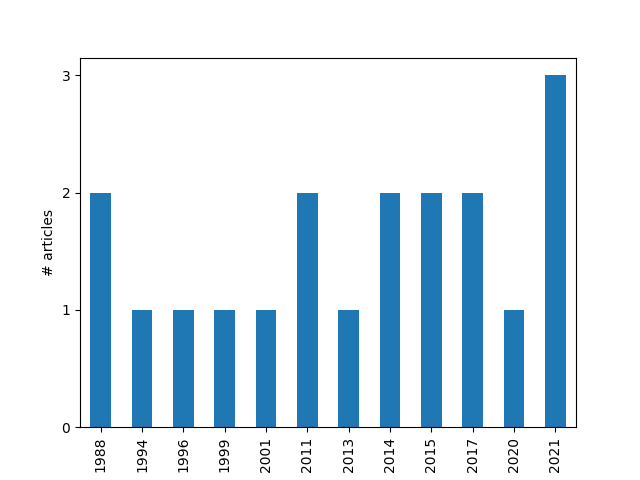
\includegraphics[width=0.8\linewidth]{articles_by_years.png}
  \caption{Статьи по годам}
  \label{fig:articles-by-year}
\end{figure}

\subsubsection{Географическое распределение публикаций}

С учётом совместных исследований лидером в данной области является США,
на долю которых приходится семь публикаций,
что составляет более трети всех рассмотренных работ (рис.~\ref{fig:countries-of-origin}).
На втором месте находится Испания с тремя статьями.
Китай, Австралия, Израиль и Чехия внесли по два исследования каждая.
В то же время Индия, Италия, Португалия, Словакия, Бельгия, Оман, Франция, Тунис, Турция и Нидерланды представлены одной публикацией каждая.

\begin{figure}
  \centering
  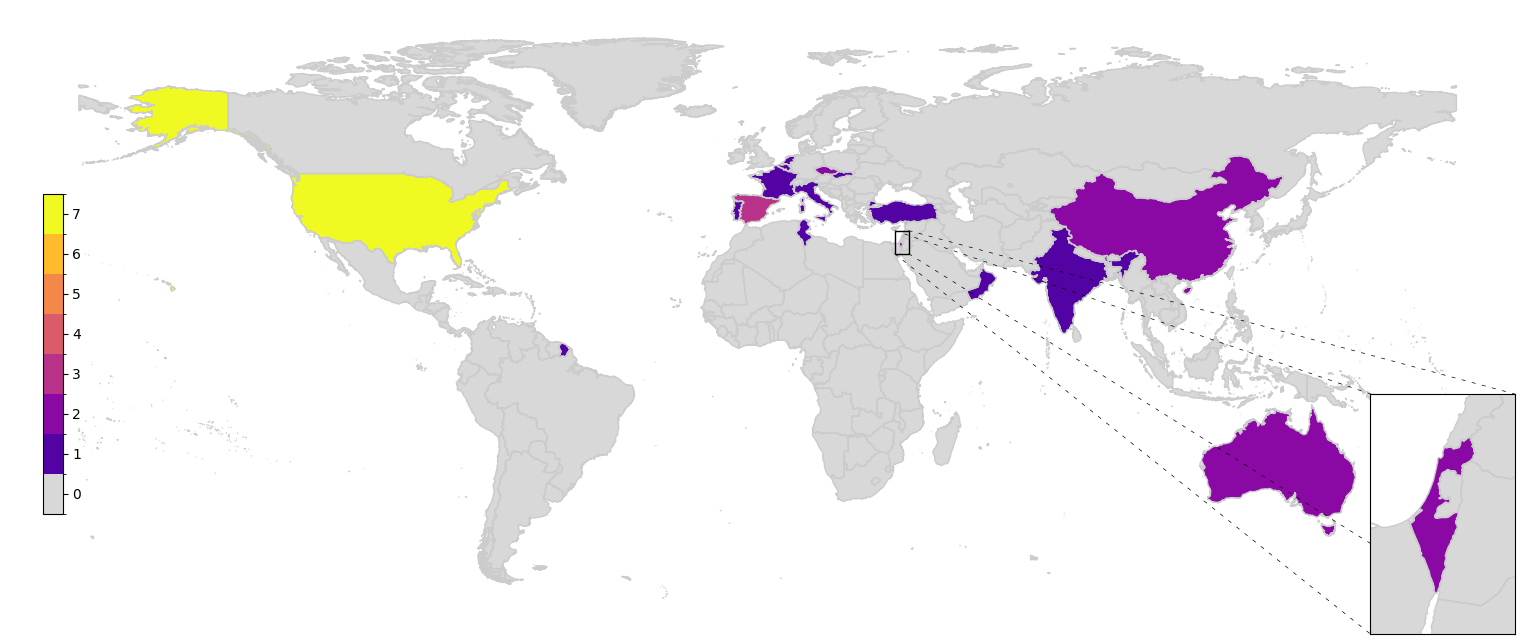
\includegraphics[width=0.8\linewidth]{countries_of_origin.png}
  \caption{Распределение по странам}
  \label{fig:countries-of-origin}
\end{figure}

\subsection{Определение текущих тенденций}

\begin{figure}
  \centering
  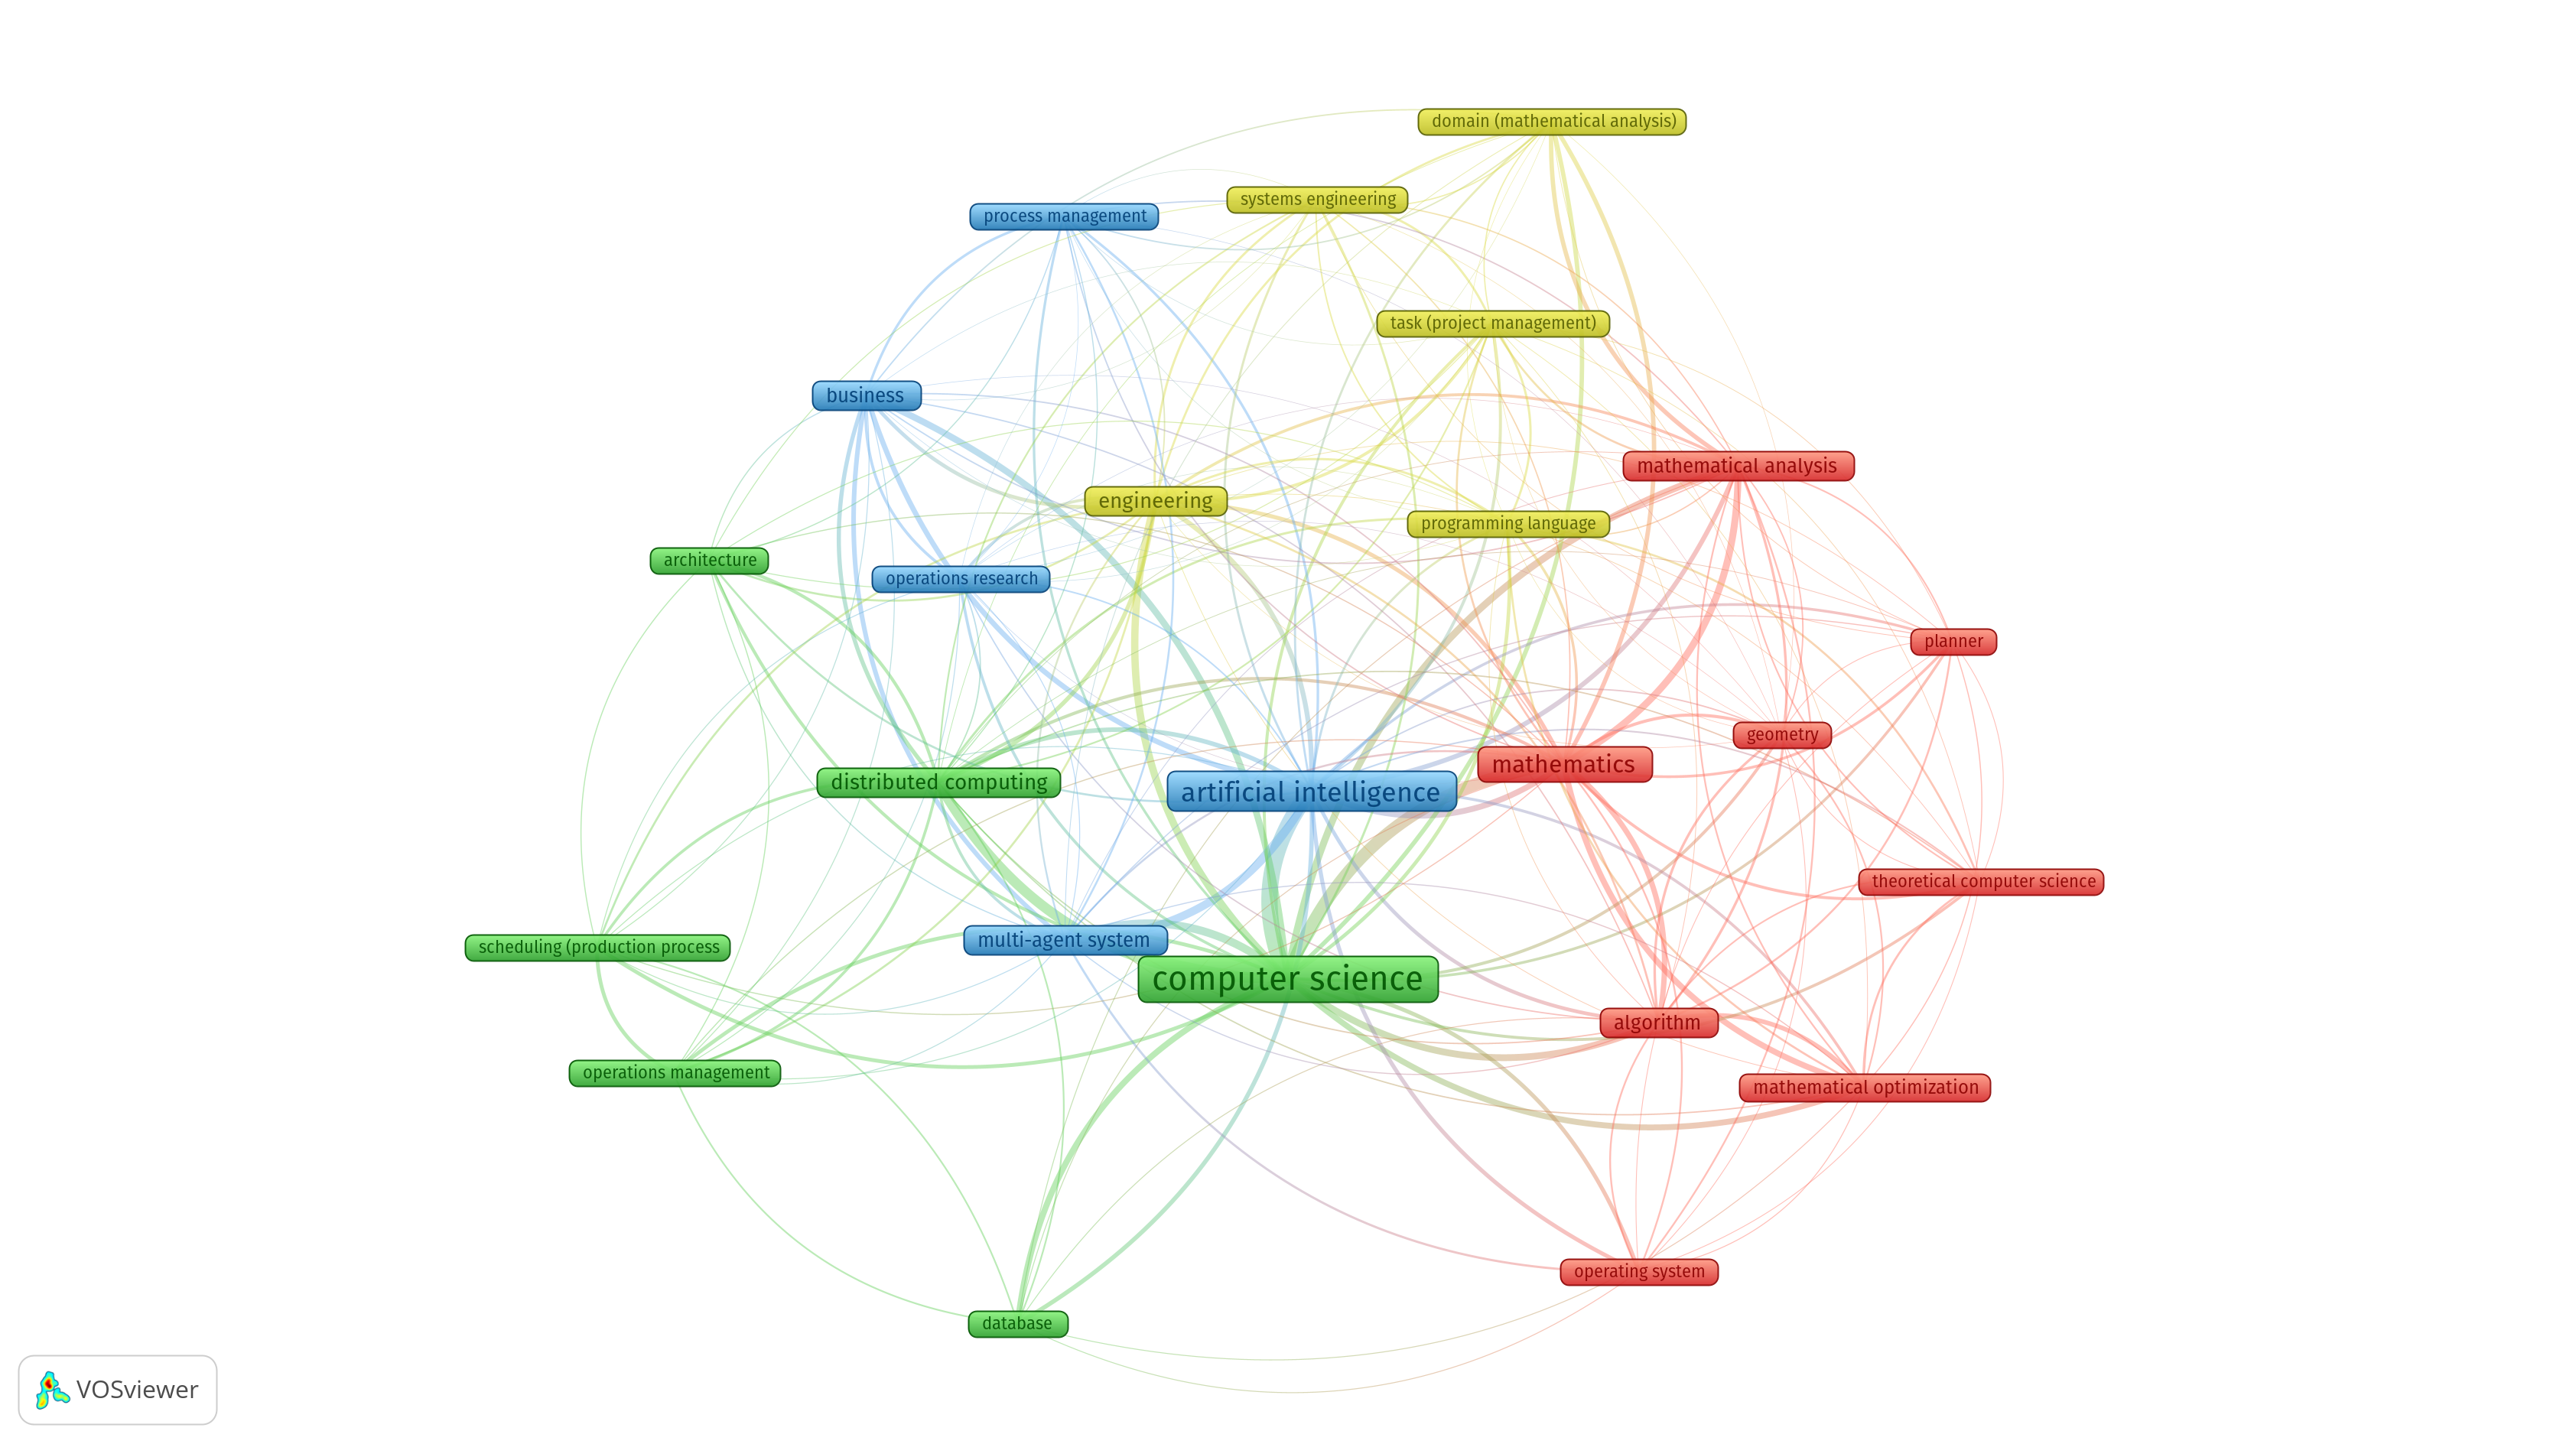
\includegraphics[width=0.8\linewidth]{co-occurence.png}
  \caption{Совместное использование ключевых слов}
  \label{fig:co-occurence}
\end{figure}

Анализируя данные, извлеченные из статей, можно выделить четыре основные области (рис.~\ref{fig:co-occurence}):

\paragraph{Математика}

Этот кластер (красный) акцентирует внимание на математическом моделировании, методах оптимизации и проектировании алгоритмов.
Существуют сильные связи между <<математикой>> и <<математическим анализом>>,
отражающие теоретические основы, а также между <<математикой>> и <<алгоритмом>>, что подчеркивает вычислительные стратегии.

\paragraph{Информатика}

Этот кластер (зеленый) сосредоточен на архитектуре систем, обработке данных и распределенных системах.
Значимые связи включают <<информатику>> с <<распределенными вычислениями>> и <<базой данных>>,
что иллюстрирует вычислительные методы для обработки данных в ресурсоемких задачах.

\paragraph{Искусственный интеллект}

Этот кластер (синий) охватывает интеллектуальные системы, принятие решений и оптимизацию процессов.
Сильные ассоциации наблюдаются между <<искусственным интеллектом>> и <<мультиагентными системами>>,
а также между <<ИИ>> и <<управлением процессами>>.

\paragraph{Инжиниринг и разработка систем}

Этот кластер (желтый) сосредоточен на внедрении и системной инженерии,
противопоставляя себя более теоретическим кластерам, описанным выше.
Существенные связи связывают <<системную инженерию>> с <<управлением задачами>> и <<математический анализ>> с <<управлением задачами>>,
подчеркивая интеграцию аналитических методов в проектирование систем.

Однако самые сильные связи --- между кластерами, особенно между математическими основами и вычислительными системами.
Связи, такие как <<математика>> и <<информатика>>, показывают, что математика является основой информатики,
в то время как <<алгоритм>> и <<искусственный интеллект>> подчеркивают интеграцию алгоритмических подходов в ИИ.
Междисциплинарные связи между <<распределёнными вычислениями>> и <<мультиагентными системами>> подчеркивают распределённые подходы в кооперативном планировании,
а связи между <<инженерией>> и <<искусственным интеллектом>> акцентируют внимание на том,
что, хотя рассматриваемые статьи в основном касаются теоретических приложений,
реальные потребности также находятся в центре внимания этих исследований.
Это не вызывает удивления,
поскольку оно отражает естественный порядок вещей в исследуемой области,
а именно — в области информатики.

\subsection{Синтез результатов}

\subsubsection{Моделирование проблемы}

\paragraph{Представление домена}

Алгоритмические подходы к разрешению конфликтов и кооперативному планированию в MAS
обычно основываются на определении структурированных доменов, в которых взаимодействуют агенты.
Эти домены моделируются с использованием формальных представлений,
таких как графы ограничений~\cite{SHARON201540,SEMIZ2021220},
иерархические сетевые задачи~\cite{FRANKOVIC20017} и архитектуры blackboard~\cite{DURFEE1988268}.
Подобные формализмы способствуют четкому определению целей,
ограничений и взаимозависимостей между агентами~\cite{GROSZ1996269}.
В качестве математических моделей часто используются задачи удовлетворения ограничений,
которые позволяют учитывать требования к принятию решений и накладываемые ограничения~\cite{KOMENDA201476}.
Благодаря этим формализмам агенты могут работать автономно, обеспечивая согласованность с общими целями.

\paragraph{Представление состояний и целей}

Подходы, основанные на моделировании состояний, позволяют агентам отслеживать их прогресс и динамически оценивать изменения в окружающей среде.
Проблемы, как правило, формулируются в виде переходов между состояниями,
где действия определяются для достижения заданных целей~\cite{CHOUHAN2015396}.
Агенты поддерживают локальные представления среды,
дополненные общими ограничениями и возможностями для согласования действий на глобальном уровне~\cite{ROSENSCHEIN1988187}.
Цели могут определяться явно как конечные состояния или неявно через функции полезности,
оценивающие эффективность выполнения задач~\cite{MA2021103823}.
Кроме того, модели часто включают вероятностные методы рассуждения для учета неопределенности,
что повышает устойчивость и надежность принятия решений~\cite{WU2011487}.

\paragraph{Временное и динамическое моделирование}

С учетом динамической природы мультиагентных систем многие подходы интегрируют временные модели
для управления изменяющейся средой~\cite{MA2021103823,LU2014215}.
Для структурирования последовательности задач и координации выполнения
в изменяющихся условиях используются рабочие процессы и событийно-ориентированные фреймворки.
Временные ограничения задают границы временных окон выполнения задач,
обеспечивая синхронизацию между агентами.
Динамические обновления посредством инкрементальных механизмов планирования позволяют адаптироваться в реальном времени,
как это наблюдается в методах с итеративным уточнением и поэтапной корректировкой планов~\cite{SEMIZ2021220}.
Эти методологии позволяют системам реагировать на непредвиденные изменения без необходимости полного перепланирования.

\subsubsection{Стратегии разрешения конфликтов}

\paragraph{Удовлетворение и расслабление ограничений}

Алгоритмы, такие как Conflict-Based Search,
решают конфликты путем итеративного уточнения решений
за счет добавления или ослабления ограничений~\cite{SHARON201540}.
Эти стратегии опираются на пошаговые оценки для эффективного разрешения конфликтов при сохранении оптимальности.
В более динамичных условиях инкрементальные корректировки позволяют системам
устранять неожиданные конфликты в реальном времени без необходимости полного пересмотра планов~\cite{KOMENDA201476}.

\paragraph{Переговоры и торги}

Подходы, основанные на переговорах, используют механизмы распределения задач,
включая модели торгов и аукционов,
для распределения ресурсов и задач между агентами~\cite{GHARRAD2021108282,FRANKOVIC20017,RABELO1994303}.
Эти методы акцентируют кооперативные взаимодействия,
в которых агенты итеративно уточняют соглашения на основе приоритетов и ограничений.
Гибкость в перераспределении задач способствует масштабируемости и способности адаптироваться к изменяющимся условиям.
Динамические корректировки и циклы пересмотра договоренностей обеспечивают устранение возникающих конфликтов в ходе выполнения задач.

\paragraph{Аргументация и мета-рассуждение}

Некоторые фреймворки включают методы аргументации,
позволяя агентам участвовать в структурированных диалогах для разрешения конфликтов~\cite{PAJARESFERRANDO201322,FERRANDO20171}.
Системы аргументации оценивают конкурирующие утверждения,
выявляют несоответствия и приходят к соглашениям через процессы мета-рассуждения.
Этот подход особенно эффективен в сценариях,
требующих объяснительного обоснования решений или согласованных действий в рамках коллективного контекста.
Моделирование обновления убеждений и корректировки предпочтений
в аргументационных механизмах способствует прозрачному принятию решений и адаптивности.

\subsubsection{Механизмы кооперации}

\paragraph{Распределенный и децентрализованный контроль}

Методы распределенного планирования составляют основу кооперативных мультиагентных систем.
Эти подходы избегают централизованного управления~\cite{DURFEE1988268,GRASTIEN2020103271,MA2021103823}
в пользу децентрализованных структур, где агенты действуют независимо,
координируясь через общие коммуникационные протоколы~\cite{ROSENSCHEIN1988187}.
Такая структура повышает масштабируемость, отказоустойчивость и надежность системы,
снижая зависимость от централизованных координаторов.
Протоколы обеспечивают обмен ограничениями и обновлениями, позволяя агентам синхронизировать действия и эффективно использовать ресурсы.

\paragraph{Декомпозиция задач и иерархии}

Методы иерархической декомпозиции задач позволяют разделять сложные проблемы на более мелкие подзадачи,
обеспечивая их параллельное выполнение и улучшенный контроль~\cite{JUNG1999149}.
Эти подходы используют многоуровневые структуры планирования,
где высокоуровневые цели определяют низкоуровневые действия.
Иерархии способствуют разрешению конфликтов за счет изоляции зависимостей внутри групп задач,
что упрощает управление взаимодействиями агентов.
Такая структура также поддерживает масштабируемость и модульное планирование~\cite{RODRIGUEZ201113005},
делая ее подходящей для крупных систем.

\paragraph{Динамические обновления и адаптация}

Механизмы динамической адаптации обеспечивают способность мультиагентных систем реагировать на изменения в окружающей среде.
Циклы обратной связи и методы итеративного обучения позволяют агентам непрерывно оценивать производительность
и корректировать планы на основе наблюдаемых результатов~\cite{LU2014215}.
Методы восстановления планов и инкрементальной корректировки повышают устойчивость системы,
сводя к минимуму сбои в ходе выполнения задач.
Эти механизмы особенно важны в динамичных доменах, где условия изменяются непредсказуемо.

\subsubsection{Оценка эффективности}

Оценка эффективности представленных методологий выявляет их сильные и слабые стороны.
Методы удовлетворения ограничений отличаются математической строгостью и масштабируемостью,
что делает их эффективными в структурированных доменах,
где ограничения могут быть четко заданы~\cite{STOLBA2017175}.
Однако в условиях высокой динамичности или неопределенности они могут требовать дополнительных адаптивных слоев~\cite{SHARON201540}.
Переговорные подходы демонстрируют гибкость и адаптивность за счет динамического распределения задач.
Итеративная корректировка и пересмотр соглашений делают их пригодными для открытых и изменяющихся сред.
Тем не менее, их зависимость от коммуникационных протоколов может вызывать накладные расходы в условиях ограниченной пропускной способности или задержек~\cite{PAJARESFERRANDO201322}.
Аргументационные фреймворки эффективны в областях, требующих обоснования решений,
обеспечивая прозрачность и доверие в коллективном принятии решений.
Однако их вычислительная сложность может быть ограничивающим фактором в масштабных системах с многочисленными агентами~\cite{FERRANDO20171}.
Кооперативные механизмы, основанные на распределенном управлении и иерархической декомпозиции,
демонстрируют высокую масштабируемость и отказоустойчивость,
что делает их эффективными в больших децентрализованных системах~\cite{MA2021103823}.
Однако они могут требовать сложных протоколов координации для обеспечения согласованности, особенно в системах с разнородными агентами~\cite{JUNG1999149}.
Методы динамической адаптации повышают устойчивость и оперативность,
делая их незаменимыми в условиях неопределенности и изменений~\cite{LU2014215}.
Однако их эффективность часто зависит от качества механизмов обратной связи
и способности балансировать исследование новых решений и использование имеющегося опыта.

\section{Обсуждение}

\subsection{Обобщение данных}

Этот обзор рассматривает стратегии разрешения конфликтов и механизмы кооперации в мультиагентных системах,
фокусируясь на моделировании, методах решения и взаимодействии.
Формальные представления, такие как задачи удовлетворения ограничений,
иерархические сети задач и временные модели, служат структурной основой~\cite{GROSZ1996269,KOMENDA201476}.
Эти методы учитывают ограничения и неопределенности, поддерживая координацию через основанное на состояниях рассуждение и обновления~\cite{STOLBA2017175,LU2014215}.

Разрешение конфликтов опирается на удовлетворение ограничений, переговоры и аргументационные структуры.
Конфликтно-ориентированный поиск уточняет решения для динамических сред~\cite{SHARON201540}.
Переговоры и торговля улучшают распределение ресурсов,
но увеличивают коммуникационные издержки~\cite{PAJARESFERRANDO201322,FRANKOVIC20017}.
Аргументационные методы повышают прозрачность, но страдают от проблем масштабируемости~\cite{FERRANDO20171}.

Кооперация достигается через распределенное управление и иерархии задач,
обеспечивая масштабируемость и отказоустойчивость~\cite{MA2021103823,JUNG1999149}.
Динамическая адаптация повышает устойчивость с помощью итеративного обучения и обратной связи~\cite{SEMIZ2021220}.

Эффективность методов зависит от условий: модели ограничений успешны в структурированных средах,
переговоры гибки в динамических сценариях, аргументация повышает объяснимость решений.
Однако остаются вызовы масштабируемости, адаптивности и вычислительных затрат,
требующие усовершенствованных критериев оценки и универсальных методологических основ.
Дальнейшие исследования должны устранить эти ограничения для создания надежных и масштабируемых решений.

\subsection{Ограничения}

Можно выделить несколько потенциальных ограничений.  

\subsubsection{Отсутствие унифицированных стандартов оценки}

Отсутствие единых кросс-доменных критериев оценки в различных исследованиях
создает проблему для проведения содержательных сравнений.
Например, одни работы делают акцент на вычислительной эффективности,
тогда как другие отдают приоритет адаптивности или стабильности.

\subsubsection{Зависимость от данных, полученных на основе симуляций}

Значительная часть представленных в рассмотренных исследованиях данных получена из симуляций,
а не из реальных внедрений. Хотя симуляции обеспечивают контролируемые условия тестирования,
они могут не полностью отражать сложности развертывания мультиагентных систем в динамических реальных средах.  

Устранение этих ограничений в будущих исследованиях за счет расширения критериев включения,
стандартизации метрик и интеграции реальных кейс-стадий позволит повысить полноту и актуальность обзора.

\chapter{Одноагентный планировщик}

Проведённый обзор существующих методов кооперации и разрешения конфликтов
в мультиагентных системах позволил выявить ключевые направления развития,
а также ограничения и пробелы в текущих подходах.
На основе полученных результатов была сформулирована архитектурная
концепция собственной системы планирования.
Следующим этапом стала разработка и реализация планировщика для одного агента,
который служит фундаментом для построения более сложной мультиагентной системы.
Этот компонент необходим не только для отладки и верификации базовых алгоритмов,
но и для обеспечения гибкости и расширяемости
при переходе к взаимодействию между несколькими агентами.
В данной главе подробно рассматривается внутренняя
структура одноагентного планировщика и принципы его функционирования\footnotemark{}.

\footnotetext{
  Результаты разработки, включая исходный код планировщика и этой статьи,
  можно найти в интернете по адресу \url{https://github.com/rudn-lab/planning-mesh-swarm/}
}

\section{Цели при разработке планировщика}

Основная причина, по которой нельзя использовать уже существующий планировщик,
заключается в том, что нам необходима гибкость и контроль над внутренней структурой,
что может быть обеспечено только своим планировщиком. Таким образом,
не будет ограничений, связанных с существующей программной архитектурой.
Цели при разработке этого планировщика были следующими:

\begin{enumerate}
  \item Гибкость --- изменения в отдельных компонентах
    должны быть легко реализуемы в процессе разработки для облегчения
    экспериментов и предотвращения возможных переписей в будущем, если текущая
    структура помешает дальнейшему развитию.
  \item Корректность --- весь код планировщика должен быть покрыт
    модульными и интеграционными тестами.
    Из-за этого быть уверенными в поведении каждого компонента,
    а также в корректности всего планировщика.
    Это также предотвратит ошибки в процессе разработки и регрессии при рефакторинге.
  \item Скорость --- планировщик должен быть достаточно быстрым для решения предоставленных задач.
  \item Расширяемость --- \jar{Application Programming Interface} (API)
    этого планировщика в виде библиотеки должен позволять потенциальному программисту
    легко определять собственные алгоритмы планирования.
\end{enumerate}

К концу разработки планировщика нам удалось успешно
достигнуть всех перечисленных целей.

\section{Выбор языка программирования}

Планировщик в этой работе был написан на языке программирования Rust~\cite{rust},
так как он обладает несколькими преимуществами по сравнению с более популярными языками,
такими как C++, Java, Python и C\#,
что делает его языком выбора для написания стабильных
и высокопроизводительных приложений. Вот эти преимущества:

\begin{itemize}
  \item \textbf{Безопасность памяти} --- система проверки заимствований в Rust гарантирует,
    что выделение и освобождение памяти всегда происходит безопасно,
    что устраняет целые классы ошибок, такие как <<двойное освобождение>>
    и <<использование после освобождения>>.
    Система проверки заимствований устраняет необходимость в сборщике мусора,
    что дополнительно увеличивает производительность и позволяет библиотекам,
    написанным на Rust, использоваться не только другими программами на Rust,
    но и программами на других языках через интерфейс внешних функций
    (\jar{Foreign function interface}, FFI).
  \item \textbf{Явная изменяемость} --- система проверки заимствований
    также контролирует способ доступа к переменным в Rust.
    Данные либо не изменяемы по умолчанию, что означает, что они не могут быть изменены и,
    следовательно, могут быть заимствованы многими функциями,
    либо они явно изменяемы, что позволяет модификации,
    но ограничивает количество заимствующих до одного.
    Это гарантирует, что данные всегда остаются консистентными,
    устраняет условия гонки и обеспечивает требуемые паттерны использования.
  \item \textbf{Низкоуровневый контроль} --- используя ключевое слово \textit{unsafe},
    Rust позволяет выполнять низкоуровневые операции,
    выходящие за пределы контроля системы заимствований,
    такие как арифметика указателей.
    Однако, случаи, когда такой низкоуровневый доступ необходим --- довольно редки.
  \item \textbf{Сильная типизация} --- алгебраическая система типов Rust
    позволяет выражать структуры данных наиболее естественным способом,
    что помогает точно определять сложные состояния приложения.
    Дополнительно, \jar{типажы} (\textit{Traits}) и \jar{обобщения} (\textit{Generics})
    помогают определять общие поведения для нескольких типов,
    что позволяет реализовать сложный полиморфизм без потери производительности.
  \item \textbf{Высокая производительность} --- Rust компилируется напрямую в машинный код,
    избегая виртуальных машин, используемых в таких языках, как Java,
    что позволяет достигать уровней производительности, сравнимых с C и C++.
  \item \textbf{Эргономичность} --- хотя Rust позволяет явным образом контролировать
    многие низкоуровневые процессы, он также имеет множество высокоуровневых абстракций,
    которые упрощают процесс написания кода.
    Еще лучше то, что многие из этих абстракций являются \jar{абстракциями без дополнительных затрат},
    поэтому они не влияют на производительность программы,
    при этом немного увеличивая время компиляции.
  \item \textbf{Экосистема Crates} --- большое и увлеченное сообщество Rust
    разработало множество качественных библиотек или \jar{Crates},
    решающих многие распространенные и не очень задачи.
  \item \textbf{Встраиваемые приложения} --- программу на Rust легко разрабатывать для встраиваемых систем.
    На самом деле, этот планировщик разработан так,
    чтобы его можно было запустить на микроконтроллере,
    что повлияло на несколько решений в процессе разработки,
    например, на необходимость интернирования~\cite{enwiki:interning} всех строк, используемых для имен.
\end{itemize}

Все эти факторы, а также высокая степень знакомства авторов с этим языком,
сделали Rust очевидным выбором для разработки планировщика.

\section{Архитектура}

Архитектура планировщика довольно проста.
Два центральных компонента — это Состояние и Действие.
Хотя Домен и Задача являются тем, что планировщик потребляет,
именно эти два компонента играют основную роль в процессе планирования.

\pc{Состояние} представляет собой всю текущую информацию о мире
в виде набора \pc{Предикатов}, которые похожи на вопросы,
на который можно ответить <<да>> или <<нет>>:
<<Находится ли коробка $b$ в местоположении $l$?>>,
<<Находится ли робот $r$ в местоположении $l$?>>,
<<Держит ли робот $r$ коробку $b$?>> и так далее\footnotemark{}.
Если состояние содержит предикат с заданными (\textit{инстанцированными}) значениями,
то этот предикат считается \textit{истинным}, но \textit{ложным} в противном случае.
Хотя строго говоря только начальное Состояние
является явно определенным пользователем,
состояния, полученные на основе начального состояния, позволяют
планировщику оценивать выражения,
включая Цель, для нахождения решения заданной Задачи.

\footnotetext{
  Возможно, было бы правильнее сказать, что Предикат
  является центральным элементом всего планировщика, поскольку он является основой
  логики планировщика. Однако они почти никогда не
  встречаются сами по себе,
  за исключением части \cd{:init} файла задачи.
  Они всегда являются частями чего-то большего, и это <<что-то большее>> является тем,
  что пользователь создает (Действия, Выражения),
  например, при использовании этой библиотеки планирования.
}

\pc{Действие} определяет преобразование Состояния мира.
Обычно это представляет собой реальное действие,
которое, например, может выполнить робот.
Оно состоит из трех компонентов:
\begin{itemize}
  \item \pc{Параметры} --- как параметры функции в языке программирования,
    они определяют, на какие Объекты действует Действие.
    Эти параметры имеют Тип, который ограничивает Объекты.
    Они связывают Предусловие и Эффект Действия.
  \item \pc{Предусловие} --- это логическое выражение, которое комбинирует
    несколько Предикатов. Если оно оценивается как \textit{истинное} в текущем Состоянии,
    то это Действие может быть применено.
  \item \pc{Эффект} --- если Действие может быть примененно к Состоянию
    с конкретными Объектами, то этот Эффект может быть
    использован для его изменения с целью перехода в новое Состояние.
\end{itemize}

\subsection{Объекты и типы}

\pc{Объект} представляет собой отображение конкретного объекта
из реального мира в упрощенное представление в Домене.
Объекты обычно делятся на две категории: Константы и обычные Объекты.
Первые присутствуют во всех Задачах для конкретного Домена,
где они определены. На практике это означает, что Константы
могут быть использованы в определении Действия или Цели.
Обычные Объекты, с другой стороны, определяются только для конкретной Задачи.
Обе категории не могут быть изменены в процессе решения, поэтому в этом планировщике
и Константы, и Объекты
объявляются, используются, хранятся и представляются одинаково.

\pc{Типы} используются для ограничения того,
какие Объекты могут быть параметрами Действия или Предиката.
Типы позволяют объявлять в Домене как общие, так и специфичные Действия и Предикаты.
Типы образуют иерархию, в верхней части которой находится тип \textit{object}.
Когда Действие или Предикат определены с конкретным Типом,
Объекты этого Типа, а также его подтипы могут быть использованы в этих конструкциях.

И Объекты, и Типы хранятся вместе в \cd{EntityStorage},
а код вне его использует \jar{дескрипторы} --- \cd{SmartHandle}.
\cd{SmartHandle} позволяет более эффективно использовать память,
так как она хранят индекс в \cd{EntityStorage}.
Дополнительно каждый \cd{SmartHandle} хранит ссылку на сам \cd{EntityStorage}.
это помогает избежать передачи \cd{EntityStorage} в каждую функцию,
где делаются запросы к системе типов.
Паттерн \jar{Interior mutability}~\cite{interiormut} в Rust,
а также стратегическое предоставление только подмножества методов,
которые есть у \cd{EntityStorage}, позволяет гарантировать,
что все дескрипторы имеют актуальную ссылку на \cd{EntityStorage},
и что его содержимое может быть изменено только во время инициализации Домена и Задачи,
а не в процессе планирования.
Такой, возможно, несколько запутанный способ хранения позволяет
эффективно запрашивать информацию о доступных Типах и Объектах,
например, получать все \cd{ObjectHandles} для конкретного \cd{TypeHandle}.

\subsection{Предикаты}

Как уже упоминалось, \pc{Предикат} похож на вопрос с ответом <<да>> или <<нет>>.
Точнее, они могут быть либо \textit{истинными}, либо \textit{ложными} в любой момент плана.
Истинность зависит от того, находится ли Предикат в Состоянии,
если да --- то он является \textit{истинным},
и, если не указано иное, предполагается, что они ложны
(за исключением случаев, когда в качестве Требования включена гипотеза об <<открытом мире>>~\cite{marks1990planning,Keet2013}).
Предикаты применяются к конкретному типу Oбъектов или ко всем Oбъектам,
что определяется Типом аргумента, который они принимают.

Структура \cd{Predicate} в планировщике тесно соответствует этому определению.
Кроме интернированного имени предиката,
она содержит список, который указывает Типы
аргументов, которые может принимать этот Предикат.
Другой список представляет фактические значения для этих аргументов.
Значения обобщены по типу \cd{PredicateValue} (предикатное значение),
что позволяет представлять различные варианты предикатов в процессе планирования\footnotemark{}.
В этой программе используются следующие варианты \cd{Predicate}:

{\sloppy
\begin{itemize}
  \item \cd{LiftedPredicate} --- эти предикаты наиболее универсальны
    из всех. Они используются внутри определения Действия,
    и, следовательно, могут содержать весь спектр значений:
    \begin{itemize}
      \item Константы --- как уже упоминалось,
        это \cd{Objects}, которые определены в Домене
        и присутствуют для всех Задач.
      \item Параметры Действия --- Объекты, которыми оперирует Действие.
      \item Связанные переменные --- поскольку планнер поддерживает выражения
        с кванторами, нам нужно представлять переменные,
        которые связывают кванторы в предикатах.
    \end{itemize}
  \item \cd{ScopedPredicate} --- эти предикаты появляются в Цели
    и отличаются от \cd{LiftedPredicates} исключением параметров Действий.
  \item \cd{GroundPredicate} --- наиболее ограниченный тип \cd{PredicateValue}.
    Эти предикаты содержат только Объекты и представляют конкретный факт о мире планирования,
    и, как таковые, появляются только в Состоянии.
\end{itemize}
}

\footnotetext{
  Поскольку предикаты обобщены по типу значения,
  это заставляет выражения, содержащие их, также быть обобщенными по этому типу значения.
  Однако более интуитивно правильным способом представления выражений является
  представление их как обобщенных по варианту самого Предиката.
  Поэтому был реализован дополнительный типаж \cd{IsPredicate}
  для предикатов с различными значениями, чтобы достичь этого.
}

В дополнение к обязательным имени, списку аргументов и списку значений,
определение \cd{Predicate} содержит два дополнительных поля,
которые не являются частью определения предиката как такового,
но которые полезны внутри этого планировщика.
\cd{EvaluationStrategy} определяет способ оценки
любого данного предиката в Состоянии.
Когда используется стратегия \cd{Equality}, то проверяется буквальное равенство
двух значений этого предиката.
Иначе, в стратегии \cd{State} проверяется, существует ли совместимый \cd{GroundPredicate} в \cd{State}.
Другим важным полем, которое присутствует на протяжении всего процесса планирования,
но остается в основном скрытым, является уникальный \cd{Marker},
который каждый предикат генерирует при создании.
Его цель --- избежать ошибочного учета или возвращения дублирующих
предикатов после преобразования логических выражений.
Например, выражение $p \veebar q$, где $p$ и $q$ --- это какие-то предикаты,
можно преобразовать в следующее выражение в \jar{Дизъюнктивной нормальной форме} (ДНФ):
$\left(p \land \lnot q\right) \lor \left(\lnot p \land q\right)$.
В этой ДНФ и $p$, и $q$ появляются дважды,
но повторения по-прежнему представляют один и тот же предикат.
Таким образом, и исходное выражение, и полученная ДНФ должны трактоваться
как содержащие только два предиката, например, для целей
построения таблицы истинности.

Из-за относительно высокой внутренней сложности
\cd{Predicate} не создается с использованием
инстанцирования или метода построения.
Вместо этого используется паттерн
\jar{Строитель} (Builder)~\cite{enwiki:builder},
точнее, паттерн \jar{Строитель с типовым состоянием} (Typestate builder).
Он использует маркерные типы для отслеживания конфигурации строителя во время компиляции,
обеспечивая корректность.
В отличие от традиционных строителей,
которые часто позволяют создать недействительные или неполные конфигурации
поскольку все методы доступны в любой момент,
Строители с типовым состоянием предотвращают это, кодируя
текущее состояние (шаг) строителя в его типе,
так что возможны только корректные цепочки методов.
Это предотвращает создание неполных объектов
и ловит ошибки конфигурации на этапе компиляции.

В случае с \cd{Predicate} строитель довольно прост,
по сравнению с описанным ниже,
но он все же заслуживает более тщательного рассмотрения, чтобы предоставить базовую реализацию.
\cd{PredicateBuilder} является обобщенным и имеет четыре состояния,
представленные \jar{нульразмерными структурами} (zero-sized structs):
\cd{New}, \cd{HasName}, \cd{HasArguments} и \cd{HasValues},
которые используются вместо обобщенного параметра.
Эти состояния представляют основные этапы создания предиката.
Первые три этапа:
\begin{enumerate}
  \item присвоение имени,
  \item определение типов аргументов и их порядка,
  \item присвоение значений аргументам.
\end{enumerate}

Последний этап раскрывает только один метод \cd{build()},
задача которого заключается в том, чтобы проверить, что значения
могут быть корректно присвоены аргументам, а затем построить сам \cd{Predicate}.
Этот метод может вернуть ошибку, если значения не соответствуют аргументам.
Примечательно, что строитель не уничтожается при присвоении значений аргументам,
вместо этого он клонируется. Это позволяет нам использовать одно и то же определение предиката
для создания нескольких предикатов с различными наборами значений.
Чтобы упростить будущий код, \cd{PredicateBuilder}, который уже имеет
аргументы, но не значения, именуется как \cd{PredicateDefinition}.

В дополнение к полной цепочке, необходимой для определения произвольного Предиката,
этот строитель предоставляет метод, который используется для создания предикатов равенства.
Он просто принимает два значения, которые должны быть сравнены,
и создает с ними \cd{Предикат}, при этом гарантируя, что
\cd{Equality} будет выбрана как \cd{EvaluationStrategy}.

\subsection{Выражения логики первого порядка}

Предикаты могут быть объединены для формирования логических выражений или \pc{Формул}.
Этот Планировщик в частности и PDDL в целом поддерживают кванторы, такие как
квантор всеобщности и существования, в выражениях,
что означает, что эти выражения представленны логикой первого порядка.
Это представляет собой ряд уникальных проблем,
поскольку нам необходимо преобразовать свободное выражение
в такую форму, с которой можно эффективно работать для рассуждений.

\subsubsection{Кванторы}

В задаче планирования \pc{Квантор} указывает,
сколько предикатов в Домене удовлетворяют открытой формуле.
\jar{Квантор всеобщности} $\forall x P(x)$ выражает,
что для каждого $x$ в Домене предикат $P$ истин,
тогда как \jar{квантор существования} $\exists x P(x)$ означает,
что существует некоторый $x$, для которого $P$ является истинным.

Для представления его в планировщике,
структура \cd{Quantifier} содержит список всех \cd{BoundVariables},
а также выражение, в котором используются эти переменные.
Каждая \cd{BoundVariable} содержит \cd{TypeHandle} и \cd{Marker},
который, в отличие от его использования в \cd{Predicate},
здесь указывает, с каким \cd{Quantifier} связана переменная;
поэтому он создается уникально для каждого \cd{Quantifier},
но может быть одинаковым для \cd{BoundVariables}.
Структура \cd{Quantifier} является обобщенной по нульразмерной структуре,
который указывает на его тип.

Для создания \cd{Quantifier} используется еще один строитель с типовым состоянием с двумя этапами.
На первом этапе задаются типы переменных,
а также выбирается тип конструируемого квантора,
предоставляя выбор между двумя методами,
которые устанавливают обобщенный параметр для самого строителя.
На втором этапе принимается \jar{замыкание} (closure), которое принимает связанные переменные
и возвращает выражение или, возможно, ошибку создания, которая унаследована при создании \cd{Predicate}.
Стоит уделить этому паттерну немного больше внимания, так как он будет часть повторяться в дальнейшем.

Задание внутреннего выражения таким образом решает несколько задач одновременно:
\begin{enumerate}
  \item Это предоставляет удобный способ использования связанных переменных в связанном выражении.
    Замыкание с \cd{BoundVariables} в качестве единственного параметра
    обеспечивает удобный доступ к ним. Код, вызывающий строителя, не должен
    как-то извлекать переменные, и тем самым нарушать эргономику.
    Вместо этого они предоставляются естественным образом.
    Это также делает неиспользование их осознанным выбором со стороны вызывающего кода,
    так как компилятор предупредит его о неиспользуемых переменных, что нужно явно игнорировать.
  \item Это задерживает построение связанного выражения.
    Не стоит строить связанное выражение сразу же
    перед передачей его в квантор, так как это не только противоречит идее использования строителя,
    который легко позволяет задерживать создание, но также может быть просто неудобно делать это сразу.
  \item Это облегчает управление ошибками.
    Создание всех объектов во время финализации строителя
    позволяет выполнять все необходимые проверки корректности в одном месте.
    Это также упрощает код, поскольку тогда только метод \cd{build()} может возвращать ошибки.
  \item Это упрощает написание кода.
    Когда используется этот паттерн, код становится проще как для написания, так и для понимания,
    что станет более понятно для более сложного строителя, например, для парсера позже.
\end{enumerate}

Во время выполнения функции \cd{build()},
\cd{TypeHandles} преобразуются в \cd{BoundVariables},
и замыкание, которое создает выражение, вызывается с ними в качестве параметров.
Поскольку связанное выражение создает Предикаты,
этот метод также может возвращать ошибки,
которые унаследованы от \cd{PredicateBuilder} или возникли во время
парсинга или при определении Домена или Задачи.

\subsubsection{Выражения}

Основным типом, который определяет выражение в коде планировщика,
является перечисление \cd{QuantifiedFormula}.
С помощью его вариантов рекурсивно поддерживаются общие логические соединители,
такие как \textit{И}, \textit{ИЛИ} и \textit{НЕ};
кванторы, используя отдельное перечисление
для кванторов всеобщности и существования;
и простой Предикат, который служит самым нижним элементом в дереве выражений.
Другие логические соединители, которые не определены явно
как варианты этого перечисления, могут быть построены с помощью
конструкторских методов, которые преобразуют их в определенные варианты.
Например, импликацию можно просто выразить с помощью основных вариантов.

Тем не менее, такое выражение невозможно эффективно обрабатывать из-за его сложности.
Хотя оно позволяет нам выразить необходимое состояние мира для использования действия
или цели планировщика, с ним существуют две проблемы:

\begin{enumerate}
  \item Кванторы перемешаны внутри выражения.
    Это затрудняет как его оценку, так и
    проверку того, какие значения должны быть подставлены в Предикаты
    при решении Задачи.
  \item Несоответствие формата.
    Наличие столь множества возможных соединителей
    позволяет выражению быть определенным с произвольной
    глубиной и шириной, что делает его сложным для быстрой оценки.
\end{enumerate}

Итак, первый шаг, даже перед тем, как такие выражения можно использовать
в планировщике, -- преобразовать их в нечто,
что имеет предсказуемую структуру и
легко обрабатывается.

Чтобы упростить работу с кванторами,
выражение преобразуется в \jar{Предваренную нормальную форму} (ПНФ),
в котором все кванторы находятся в \jar{префиксе} перед выражением,
а оставшаяся часть --- \jar{матрица} --- не содержит кванторов.
Это обычно трехступенчатый процесс:

\begin{enumerate}
  \item Преобразовать формулу в \jar{Нормальную форму отрицания} (НФО);
  \item Переименовать все связанные переменные,
    чтобы имена были уникальными для всех кванторов;
  \item Переместить все кванторы перед выражением.
\end{enumerate}

Однако из-за того, как определены и используются \cd{BoundVariables},
можно пропустить второй шаг
и сразу перейти к перемещению кванторов на передний план после преобразования формулы в НФО.

На первом шаге формула изменяется таким образом,
что отрицания либо исчезают, либо применяются исключительно к предикатам.
Это достигается с помощью рекурсивной формулы,
которая применяет \jar{Законы де Моргана}, чтобы переместить отрицания внутрь.
Результирующий НФО в планировщике представлен отдельным перечислением,
которое почти полностью соответствует \cd{QuantifiedExpression}, но не содержит
вариант \cd{Not} и не имеет отдельного варианта \cd{Predicate}.
Вместо этого оно содержит дополнительное перечисление \cd{Primitives},
которое представляет либо \cd{Predicate}, как есть, либо его негативную версию.
Использование этой дополнительной структуры данных утверждает на этапе компиляции,
что выражение действительно находится в НФО.

Второй шаг преобразует этот НФО в настоящий ПНФ.
Обычно это делается синтаксически,
путем применения конкретных правил эквивалентности,
например, $\left(\forall x \phi\right) \land \psi \equiv \forall x \left(\phi \land \psi \right)$.
В планировщике используется альтернативный метод,
путем обхода дерева выражений с использованием \jar{поиск в глубину}.
Каждый раз, когда встречается \cd{Quantifier},
его тип и связанные переменные добавляются в список префикса
и заменяются в дереве на связанное выражение, которое он содержал.
Это приводит к корректному ПНФ, потому что несколько кванторов \textit{вложены} друг в друга,
то есть они применяются только к своему привязанному выражению.

Тем не менее, такое преобразование оставляет матрицу в свободной форме.
Чтобы сделать ее единообразной и предсказуемой, нам нужно применить дополнительные преобразования.
Совершенная ДНФ (СДНФ), которая содержит все предикаты в каждом из своих конъюнкций,
достигает обеих этих целей, а также предоставляет уникальное преимущество
для алгоритма \jar{инстанцирования}, о котором написано ниже.

СДНФ можно прочитать из таблицы истинности выражения,
поэтому первым шагом здесь является ее построение.
Таблица истинности не учитывает конкретные значения Предикатов,
а только то, какие Предикаты присутствуют в выражении.
Поэтому можно оценить выражение для каждой перестановки
истинных и ложных Предикатов, чтобы построить эту таблицу.
Затем создается конъюнкцию для каждой комбинации Предикатов,
которая делает формулу истинной,
добавляя в эту конъюнкцию каждый Предикат, который
был истинным в своем исходном виде
или его негативную версию, если он был ложным.
Уже существующий тип \cd{Primitives}
используется для представления этих двух вариантов,
однако сами конъюнкции не представляются отдельными структурами \cd{And} и \cd{Or},
вместо этого используюется структура множества из стандартной библиотеки Rust,
которые храним в новой структуре \cd{Dnf}.
Это снова подтверждает на этапе компиляции,
что выражение действительно находится в СДНФ.

При использовании их вместе, эти два подхода дают нам
\jar{Предваренную дизъюнктивную нормальную форму} (ПДНФ),
которое представлено как структура \cd{Pdnf}.
Она содержит префикс в виде списка \cd{Quantifiers} и матрицу в виде \cd{Dnf}.
Матрица, а значит и вся структура \cd{Pdnf}, является обобщенной по типу \cd{Predicate},
как и изначальное выражение.

\subsection{Действия}

Как уже было упомянуто ранее,
\pc{Действие} определяет преобразование состояния мира.
Это единственный способ перехода между состояниями,
и, следовательно, единственный способ решения задачи планирования.
Кроме имени, структура \cd{Action} содержит
список \cd{TypeHandles}, которые представляют аргументы для \cd{Action},
так же, как они представлены в \cd{Predicate};
для определения Предусловия используется \cd{Pdnf}, содержащаий \cd{LiftedPredicate},
а специальный тип \cd{ActionEffect} представляет Эффект,
который это действие может оказать на состояние.
Использование \cd{TypeHandles} для задания аргументов
и создание \cd{Pdnf} уже подробно описано,
поэтому единственным новым элементом в этом определении является \cd{ActionEffect}.

По необходимости Эффекты, которые может вызвать действие, ограничены
по сравнению с диапазоном, который может использовать Предусловие.
При изменении состояния не может быть неопределенности,
поэтому все, что можно упростить до выражения с \textit{ИЛИ},
запрещено. Квантор существования тоже запрещен.
Поэтому перечисление \cd{ActionEffect} позволяет использовать
соединитель \textit{И}, универсальный квантор, Предикат,
который может быть негативным, и специальное выражение \textit{when} (когда).

Выражение \textit{when} позволяет добавить дополнительные условия
непосредственно к Эффектам Действия.
Оно состоит из двух частей:
условия, которое может использовать логические связки,
из \cd{QuantifiedExpression},
и Эффекта, который рекурсивно использует \cd{ActionEffect} для фактических
изменений, которые нужно внести в состояние.
Ниже подробно рассказывается, как вычисляются и применяются Эффекты,
но прямо сейчас для выражения \textit{when} важно следующее.
При обработке Эффектов сначала оценивается условие
в текущем Состоянии, что легко сделать, так как на тот момент будет доступен
хотя бы один возможный способ, как это действие может быть инстанцированно в конкретном состоянии.
Если условие истинно, то предикаты в Эффекте
добавляются в полный список изменений, которые это действие вызывает,
или игнорируются в противном случае.

Для построения \cd{Action} используется еще один строитель с типовым состоянием.
Этот строитель сочетает идеи из двух предыдущих примеров.
Он определяет типы аргументов, для этог Действия, как \cd{PredicateBuilder},
и он определяет как Предусловие, так и Эффект с помощью замыканий,
которые принимают \cd{TypeHandles} и возвращают соответствующие выражения,
как \cd{QuantifierBuilder}.
Во время финализации в методе \cd{build()},
поочередно вызываются замыкания для создания Предусловия и Эффекта.
Если ошибок не возникло, то создается новое действие.
Если же что-то пошло не так при создании,
будь то ошибка предиката или ошибка парсинга,
финализация прерывается, и возвращается результатирующая ошибка.

\subsection{Состояние}

Структура \pc{State} определяет текущую истинную информацию о мире.
Это можно просто представить в планировщике набором \cd{GroundPredicates}.
Однако здесь используется оптимизацию,
которая, несмотря на свою простоту, значительно ускоряет поиск предикатов.
Вместо использования простого множества, которое содержит все истинные \cd{GroundPredicates},
они хранятся в ассоциативном массиве,
который использует имя предиката и количество параметров в качестве ключа,
а в качестве значения --- множество соответствующих предикатов.
Это позволяет избежать поиска по всем предикатам в состоянии.

Для создания \cd{State} не используется специальный строитель.
Вместо этого все истинные предикаты передаются в конструкторную функцию в виде множества.
Во время выполнения эта функция преобразует набор в эту оптимизированную структуру.

\subsection{Домен и проблема}

Структуры \pc{Domain} и \pc{Problem} в целом соответствуют
значению и определению домена и проблемы из PDDL.
Однако некоторые конструкции, такие как \jar{Ограничения} и \jar{Метрики},
исключены, так как они не так часто используются в планировании
и могут усложнить процесс планирования без явной пользы.

\pc{Домен} описывает, какие предикаты могут описывать состояние мира,
какие константы существуют в этом мире
и какие действия могут изменять его состояние и при каких условиях.
Структура \cd{Domain} состоит из имени, набора \jar{Требований},
которые определяют, какие аспекты PDDL необходимы для работы с этим доменом\footnotemark{},
\cd{EntityStorage}, который хранит как Типы, так и Объекты,
\cd{NamedStorage} для определения предикатов и еще одного \cd{NamedStorage} для действий.
Предикаты хранятся в неполной форме определения \cd{PredicateDefinition},
так как процесс их создания требует знания как типов аргументов,
так и значений, которые они будут принимать.
Однако в PDDL в декларации \cd{:predicates} дается только список аргументов с их типами,
поэтому финализация предиката откладывается до тех пор,
пока не будут получены значения, например, в определении действия или в части \cd{:init} проблемы.

\footnotetext{
  На момент написания этого текста, разработанный планировщик поддерживает большинство распространенных Требований.
  Однако он не поддерживает \pc{Fluents}, \pc{Durative actions},
  \pc{Derived predicates}, \pc{Preferences}, \pc{Constraints} и \pc{Action costs},
  так как они не так часто используются, трудны для реализации
  и не являются необходимыми для работы планировщика.
}

\pc{Задача} составляет вторую часть задачи планирования.
В Домене выражаются глобальные аспекты задачи,
такие как: какие Действия можно выполнить
и какие Типы объектов существуют в мире, в котором происходит планирование.
Задача же конкретизирует это, определяя, какие Объекты существуют,
что о них известно, и, наконец, какая цель должна быть достигнута.
Чтобы представить это в коде, помимо имени и имени домена,
структура \cd{Problem} содержит тот же \cd{EntityStorage},
который содержит дополнительные объекты, специфичные для данной проблемы,
помимо общих Констант, а также тот же \cd{NamedStorage} для действий.
Главное отличие от домена заключается в том,
что она хранит начальный \cd{State}
Цель, определенную как \cd{Pdnf} с \cd{ScopedPredicates}.
Важно, что цель не определяется как еще одно состояние,
а как выражение, которое должно быть истинным, чтобы планировщик завершил свою работу.

Для создания как \cd{Domain}, так и \cd{Problem}
используются два дополнительных строителя с типоавым состоянием.
Эти строители работают подобным образом, как и предыдущие строители.
За исключением указания требований,
единственный способ добавить новые типы, объекты, предикаты и т.д.
--- это использовать замыкания, как при определении Предусловия в Действии.
Однако эти замыкания немного сложнее.
Во-первых, строители передают им больше параметров,
например, при добавлении новых действий строитель передает
список указанных требований, \cd{ObjectStorage} и \cd{EntityStorage}
(которые являются двумя различными типажами, реализуемыми \cd{EntityStorage},
что позволяет более гибко управлять тем, что может делать вызывающий код),
\cd{NamedStorage} для определения предикатов
и изменяемый \cd{NamedStorage} для действий,
который изначально пустой и должен быть заполнен вызывающим кодом.
Этот пример также показывает,
что не все замыкания теперь возвращают результат.
Только при определении Цели используется замыкание,
которое возвращает \cd{QuantifiedFormula} или ошибку.
Другие замыкания не возвращают ничего при отсутствии ошибок,
вместо этого они модифицируют изменяемый параметр.
Это скрывает внутренние детали реализации хранилища
и не обременяет вызывающий код определением этих деталей самостоятельно.

\subsubsection{Парсинг}

Структуры \cd{Domain} и \cd{Problem} являются основными типами,
создаваемыми при чтении и парсинге соответствующих файлов PDDL.
Парсинг самого языка выходит за рамки данной работы,
поэтому эта задача решается уже существующей библиотекой \texttt{pddl}~\cite{pddl-crate}.
Эта библиотека позволяет парсить PDDL 3.1 на основе документации,
предоставленной Planning.Wiki~\cite{planning-wiki} и \textcite{kovacs2011complete}.

Файл парсится в структуру данных,
которая близка к \jar{Формe Бэкуса-Наура} (БНФ)~\cite{bnf} языка,
но она далека от того, чтобы быть полезной,
поэтому нам необходимо преобразовать её в собственные типы планирощика.
Благодаря рекурсивной природе БНФ и используемых типов, это довольно просто сделать.
Не будем вдаваться в детали этого процесса, но важно отметить,
что в ходе преобразования проверяется, что конструкции,
используемые для определения действий и цели, соответствуют указанным Требованиям.
Таким образом, не приходится верить, что файлы Домена и Проблемы созданы правильно,
потому что происходит отдельная проверка.
Поскольку не все алгоритмы планирования могут быть применены к каждому Домену,
гарантируется, что Требования правильно отражают содержимое Домена,
чтобы позже проверять их перед запуском алгоритмов планирования.

\section{Решение Проблемы}

Решении Проблемы состоит из двух основных алгоритмических компонент.
Первый компонент определяет способ приведения действия к конкретным объектам,
определённым в решаемой задаче --- \jar{инстанцирование}.
Это позволяет нам применить Эффект Действия к Состоянию,
добавляя или удаляя конкретные Предикаты из него.

Второй компонент --- это конкретная стратегия поиска,
используемая для нахождения пути через изменения Состояния.
В данной работе используется алгоритм A\*~\cite{astar} с эвристиками,
основанными на поиске в \jar{Граф планирования с упрощением}
(Relaxed Planning Graph, RPG)~\cite{BLUM1997281,Hoffmann_2001,bryce2007planninggraph}.
Однако используемый API достаточно гибкий,
чтобы поддерживать широкий спектр алгоритмов поиска и эвристик.

\subsection{Конкретизация Действия}

Алгоритм того, как Действие может быть применено к состоянию, можно описать следующим образом.
Сначала необходимо проверить, выполняется ли его Предусловие в текущем состоянии.
Это усложняется тем, что Предикаты, описывающие состояние,
являются \jar{инстанцированными}, что означает,
что их значения являются конкретными Объектами или Константами,
определёнными для этой Проблемы.
В то время как Предикаты в Предусловии действия \jar{обобщены}
--- они не являются конкретными, и, помимо констант, содержат переменные
в виде параметров Действия как значения.
Хотя параметры Действия ограничены их Типом, 
они могут быть инстанцированы несколькими Объектами.
Поэтому нужно найти такую комбинацию Объектов,
которая при подстановке этих Объектов в соответствующие параметры приведёт
Предусловие к \textit{истине}. Может быть несколько таких комбинаций или ни одной.
Если не существует ни одной подходящей подстановки,
это значит, что Действие не может быть применено к Состоянию.
Однако, если хотя бы одна такая комбинация найдена, нужно инстанцировать Эффект этого Действия,
потому что параметры Действия появляются и в них.
Это даёт список команд для изменения состояния (\cd{ModifyState}),
которые представляют собой простые команды для добавления или удаления
конкретных инстанцированных Предикатов из Состояния.

\subsubsection{Конкретизация Предусловия}

Для того чтобы проверить, выполняется ли Предусловие Действия в данном Состоянии,
необходимо реализовать механизм, который преобразует \cd{LiftedPredicates},
содержащие параметры действия, ограниченные Типами,
а также связанные переменные в кванторах, в \cd{GroundPredicates},
которые содержат только конкретные Объекты.
Для этого используется метод \cd{ground\_action()}, определенный для \cd{State}.
В этом методе каждая конъюнкция из матрицы ПДНФ Предусловия обрабатывается отдельно.
Это возможно сделать, потому что, как было сказано ранее,
алгоритм преобразования свободного выражения в ПДНФ создает полную СДНФ в матрице,
в которой все Предикаты присутствуют в каждом выражении.
Это также гарантирует, что все параметры Действия присутствуют в каждом выражении.
Это позволяет нам не беспокоиться о пропущенных параметрах.

Конъюнкция содержит несколько Предикатов, некоторые из которых могут быть отрицательными.
Для каждого положительного Предиката можно просто,
с какими объектами он встречается в данном Состоянии.
Это дает нам отображение от \cd{LiftedValues} (параметры действия и связанные переменные)
к нескольким Объектам, для которых этот предикат может быть оценен как \textit{истина};
Это отображение является инстанцированием отдельной конъюнкции,
а в коде оно называется \cd{Grounding}.
Для отрицательных Предикатов добавляется дополнительный шаг:
нам нужно найти все Объекты, для которых внутренний положительный Предикат
не может быть \textit{истинным}.
Этого можно достигнуть, \textit{инвертируя} положительное отображение:
вычитае положительное отображение из полного множества Объектов,
которые может принять конкретный параметр Действия или связанная переменная квантора.
Результатом этого будет отображение для отрицательного Предиката.
Для каждого Предиката в конъюнкции, получается \cd{Grounding}, а затем их объединение
является общим \cd{Grounding} для всей конъюнкции.
Если один и тот же \cd{LiftedValue} встречается в нескольких Предикатах
используем пересечения множеств, что гарантирует,
что все Предикаты будут истинными вместе.

На следующем шаге необходимо учесть префикс,
чтобы дополнительно уменьшить множество возможных \cd{Grounding}.
Для успешной оценки префикса необходимо убедиться,
что, в случае универсального квантора,
\cd{Grounding} содержит полное множество объектов для его связанной переменной,
а в случае экзистенциального квантора --- что оно содержит хотя бы один объект.
Однако префикс может содержать оба типа кванторов,
поэтому необходимо также учитывать их порядок.
Это требует проверки всех комбинаций связанных переменных.
Для каждой допустимой комбинации строится отображение от связанных переменных
к соответствующим объектам и проверяем, содержится ли оно в \cd{Grounding},
рассматривая вариант \cd{BoundVariable} в перечислимой структуре \cd{LiftedValue}.
Если все комбинации успешны, это означает,
что конъюнкция \textit{истинна} при условии префиксом,
и ее \cd{Grounding} добавляется в набор результатов функции.
Перебор всех возможных комбинаций --- неоптимален,
но это допустимо по следующим двум причинам:
\begin{enumerate}
  \item Кванторы редко встречаются в выражениях,
  \item Процесс проверки всех пермутаций прерывается,
    когда одна из них не проходит,
    что позволяет избежать лишних вычислений в случае,
    если конъюнкция не \textit{истинна} с данным префиксом.
\end{enumerate}

После этого удаляются связанные переменные из \cd{Grounding},
а затем объединяем все решения для отдельных конъюнкций в одно множество,
что является полным инстанцированием Предусловия.
Это дает нам несколько <<параллельных>> способов преобразования
обобщенного Действия в инстанцированное Действие.
В случае, если это множество пусто, можно сделать вывод,
что это Действие не может быть инстанцированно в текущем состоянии,
и не продолжаем с инстанцорованием его Эффекта.

\subsubsection{Конкретизация и применение Эффекта}

Следующий шаг генерирует список вариантов \cd{ModifyState},
которые затем используются для изменения Состояния.
Для этого используется полученное на предыдущем шаге \cd{Grounding},
чтобы сначала уплощать, а затем инстанцировать \cd{LiftedPredicates} в Эффекте Действия.
Для этого применяется метод \cd{ground\_effect()}.
В этом методе, для каждого <<параллельного>> \cd{Grounding},
рекурсивная структура \texttt{ActionEffect} обрабатывается,
и когда встречается \cd{Primitive} с \cd{LiftedPredicate},
он преобразуется в набор \cd{GroundPredicates}
для каждой комбинации параметров Действия и связанных переменных,
присутствующих в нем.

Вся структура уплощается в процессе этого преобразования,
что легко сделать, так как все соединители в ней представляют собой
логическую конъюнкцию.
Полученные \cd{Primitives} затем оборачиваются в варианты
перечисления \cd{ModifyState},
чтобы лучше передать желаемые модификации.
Как уже упоминалось, если встречается выражение \textit{when},
сначала оценивается условие в текущем Состоянии,
и если оно выполняется как \textit{true}, то продолжается уплощение его Эффекта.

К концу алгоритма получается набор наборов \cd{ModifyState}.
Они используются для изменения того, какие предикаты хранятся в текущем состоянии.
Более конкретно, \cd{Add} вариант добавляет \cd{GroundPredicate}
в \cd{State}, а \cd{Del} убирает соответствующий \cd{GroundPredicate}.
Эта операция идемпотентна, что значит,
что результат удаления несуществующего Предиката --- Состояние без него,
а добавление уже существующего Предиката --- Состояние,
где этот Предикат встречается только один раз.

\subsection{Поиск в графе состояний}

Типажы \cd{Solver} и \cd{Heuristic} составляют основу API,
которое позволяет планнеру поддерживать различные алгоритмы поиска и эвристики.
Оба эти типажа определяют метод \texttt{can\_solve()},
который принимает список Требований Домена и возвращает \cd{bool},
которое указывает, способен ли конкретный решатель или эвристика
обработать необходимые конструкции PDDL.

В дополнение к этому, \cd{Heuristic} также определяет метод \cd{prepare()},
который предварительно вычисляет значения,
необходимые для корректной и эффективной работы эвристики в ходе вычислений,
а также метод \cd{call()}, который оценивает Состояние.
Метод \cd{prepare()} необходим для эвристик,
которые требуют дополнительных вычислений до основного цикла планирования,
как, например, $h\_{add}$ или $h\_{max}$, 
для которых сначало нужно вычислить RPG.

Типаж \cd{Solver} имеет только один дополнительный метод --- \cd{solve()},
который принимает объекты \cd{Problem} и \cd{Heuristic},
и возвращает список из \cd{GroundAction},
состоящих из имени Действия и конкретных Объектов, с которыми оно было инстанцировано.
Оба типажа также определяют ассоциированный тип ошибки.
Конкретное определение типа зависит от вызывающего кода и представляет собой ошибки,
которые могут возникнуть в процессе подготовки эвристики или планирования соответственно.

\section{Экспериментальные результаты}

Для тестирования производительности Планировщика.
был подготовлен и выполнен набор тестов.
Основной целью являлась проверка производительности
Планировщика, а также его способность производить
корректные планы при обработке выражений с кванторами,
сложными логическими условиями и большим количеством объектов в Домене и Проблеме.
Эти тесты производительности играли дополнительную роль стресс-тестов системы.
Они позволили количественно оценить производительность
реализованного алгоритма планирования и выявить узкие места в архитектуре.

\begin{table}
  \centering
  \begin{footnotesize}
  \caption{Результаты тестов}
  \label{tab:benchresults}
    \begin{longtable}{|c|c|c|c|c|c|}
    \hline
      Название & Объекты & Предикаты & Действия & Кванторы & Ср. время (из 1000)\\
    \hline
    \hline
    simple & 4 & 4 & 3 & Нет & 83.410 µs\\
    \hline
    mini-warehouse & 7 & 5 & 4 & Да & 5.3849 ms\\
    \hline
    move-and-push & 26 & 6 & 8 & Нет & 670.39 ms\\
    \hline
  \end{longtable}
  \end{footnotesize}
\end{table}

Как видно из таблицы~\ref{tab:benchresults},
производительность одноагентного планировщика варьируется
в зависимости от сложности задач и используемых языковых конструкций.
В тесте \textit{simple} использовался минималистичный домен с тремя действиями,
четырьмя предикатами и базовыми STRIPS-операторами.
Цель состояла в том, чтобы переместить коробку
из одной комнаты в другую.
Эта задача была решена за в среднем 83.4 микросекунды,
что подтверждает высокую эффективность планировщика
в условиях простых, хорошо структурированных задач.
Следующий тест, \textit{mini-warehouse}, был направлен на проверку поддержки
более сложных конструкций PDDL: кванторов и условных эффектов.
Домен включал очистку смежных локаций,
а также управление несколькими объектами и их перемещением.
Несмотря на возросшую сложность, среднее время решения составило около 5.38 миллисекунд,
что указывает на приемлемую вычислительную нагрузку
при использовании расширенных возможностей языка.
Тест \textit{move-and-push} представлял собой наиболее сложный случай.
Он основан на модифицированном домене, описывающем игру Sokoban~\cite{enwiki:sokoban}.
В этом Домене используются отрицательные и дизъюнктивные предусловия,
большое количество объектов, а также сложные зависимости между ними.
Целью задачи было достижение конечного положения агента и объекта,
обходя препятствия и используя различные типы взаимодействия с объектами.
Среднее время решения составило 670.4 миллисекунды,
что отражает экспоненциальный рост сложности поиска в условиях
большого количества объектов и сильно разветвлённого пространства состояний.
Хотя этот показатель заметно выше предыдущих,
следует подчеркнуть, что увеличение времени обусловлено
в первую очередь самой структурой задачи и экспоненциальным ростом
пространства поиска --- а не недостатками реализации.

Основная сложность в этой задаче заключается в выборе эвристики:
она оказывает большое влияние на то, какую часть пространства состояний необходимо
просматривать.
В зависимости от того, как именно растет дерево состояний конкретной задачи,
изменяется эффективность используемых эвристик,
поэтому возможно, что текущая эвристика лучше работает для простых задач,
не имеющих большого числа объектов или сложных Предусловий, использующих кванторы.
Тем не менее, при переходе к более насыщенным задачам с высоким числом
взаимозависимых объектов и выраженной структурой причинно-следственных связей,
становится особенно актуальным применение более информативных и строгих эвристик.
Одной из таких является эвристика \jar{Landmark Cut}~\cite{lmcut} (LMCut),
которая основывается на последовательной оценке стоимости
достижения обязательных \jar{сечений} (cut) --- множеств действий,
необходимых для выполнения хотя бы одной из оставшихся целей.
В отличие от эвристик, основанных на удалении негативных эффектов,
таких как $h_{add}$ или $h_{max}$,
эвристика LMCut сохраняет допустимость оценки,
что особенно важно при построении оптимальных планов.
Кроме того, она способна точнее учитывать стоимость действий
в условиях, когда цели зависят от труднодостижимых промежуточных состояний
или могут быть достигнуты различными путями с различной ценой.
Несмотря на большую вычислительную нагрузку на каждом шаге,
применение LMCut может существенно сократить общее число расширяемых состояний
и повысить качество планов в задачах с высоким уровнем логической насыщенности.
Рассматривается возможность интеграции этой эвристики в архитектуру планировщика
в качестве альтернативного режима для задач, требующих строгой оценки стоимости.

Несмотря на неоптимальный выбор эвристика,
результаты демонстрируют, что предложенная реализация
эффективно справляется с широким спектром задач ---
от простых до высокоуровневых,
а также подтверждают пригодность архитектуры планировщика
для использования в реалистичных сценариях с различной степенью сложности.

\chapter{Мультиагентный планировщик}

Предыдущая глава была посвещена разработке и функционированию одноагентного планировщика,
который составляет основу для мультиагентного планировщика, представленного в этой главе.
Одноагентный планировщик, сосредоточенный на формулировке целей,
последовательности действий и эффективном исследовании осуществимых планов,
предоставляет базовые механизмы, которые адаптируются и расширяются в мультиагентной среде.

Однако с переходом к планированию с участием нескольких автономных агентов
сложность задачи существенно возрастает.
Каждому агенту необходимо не только решать свои индивидуальные цели,
но также координировать действия, обмениваться информацией
и, при необходимости, корректировать свои действия в ответ на планы других.
В данной главе представлен мультиагентный планировщик,
основанный на архитектуре одноагентного планировщика
и дополненный механизмами координации,
приоритезации целей и обмена информацией.

Мультиагентный планировщик предполагает,
что все агенты обладают общими знаниями о предметной области,
что позволяет им опираться на единое представление
о среде и задачах. Каждый агент осуществляет планирование независимо,
при этом обмениваясь планами и обновлениями с другими агентами
посредством распределённого коммуникационного протокола.
Такой децентрализованный процесс планирования обеспечивает гибкость,
устойчивость и масштабируемость, делая систему подходящей для сложных
реальных сценариев, таких как рои роботов или распределённые логистические сети.

\section{Модель планирования и архитектура системы}

Модель планирования следует формализму, подобному STRIPS~\cite{FIKES1971189}:
типизированные объекты, детерминированные действия,
пропозициональные описания состояний
и классическое достижение целей,
унаследованные от одноагентного планировщика.
Все агенты наблюдают одно и то же начальное состояние и спецификацию домена,
но получают различные множества целей.
Ключевым моментом является то, что агенты реализованы как независимые сущности,
каждая из которых оснащена собственной экземпляром
планировщика, соответствующего API на языке Rust, основанному на типажах.

В частности, система планирования построена вокруг
типажов \cd{Solver} и \cd{Heuristic}, представленных в предыдущей главе.
Они определяют модульный и расширяемый интерфейс
для реализации новых алгоритмов поиска и эвристических стратегий.
Оба типажа включают метод \cd{can\_solve()},
который проверяет, способен ли данный планировщик обрабатывать
необходимые особенности домена (такие как условные эффекты или кванторные выражения).
Типаж \cd{Heuristic} дополнительно определяет метод \cd{prepare()}
для предварительной обработки таких структур,
как \jar{Граф планирования с упрощением}
(Relaxed Plannig Graph, RPG)~\cite{BLUM1997281,Hoffmann_2001,bryce2007planninggraph},
и метод \cd{call()} для оценки конкретного состояния.
Типаж \cd{Solver} инкапсулирует основную логику планирования
через метод \cd{solve()}, который принимает \cd{Problem} и \cd{Heuristic}
и возвращает \cd{Plan}, содержащий список \cd{GroundActions},
каждое из которых определяет имя действия и конкретный набор привязанных объектов.
Такая абстракция позволяет разработчикам гибко заменять и комбинировать
решатели и эвристики, сохраняя при этом единый интерфейс.

\section{Достижимость целей и приоритезация}

Перед началом планирования каждый агент выполняет эвристический анализ достижимости
путём построения RPG из общего начального состояния.
Этот граф распространяет положительные эффекты действий, игнорируя эффекты удаления,
тем самым аппроксимируя, какие предикаты
--- а следовательно, и какие цели --- могут быть достижимы.
Цели, отсутствующие в множестве достижимых по релаксации, помечаются как потенциально недостижимые.
Однако данный процесс носит консервативный характер и не гарантирует
выявление всех недостижимых целей из-за своих упрощений.
Поэтому агенты не отбрасывают такие цели полностью, а лишь понижают их приоритет в планировании.

Для управления конкурирующими задачами и ограниченными ресурсами планирования
в планировщик интегрирована приоритезация целей.
Каждый агент назначает приоритеты целям на основе нескольких критериев:
оценочной стоимости достижения (вычисляемой по RPG),
собственных предпочтений или функции полезности,
а также количества других агентов, разделяющих данную цель.
Последний критерий способствует кооперативному поведению
и помогает разрешать неоднозначности в частично пересекающихся множествах целей.
Важно отметить, что приоритезация целей используется исключительно как эвристика поиска;
она влияет на порядок планирования, но не нарушает \jar{корректность},
которая здесь определяется строго как сохранение корректности плана
в отношении достижения целей и логической непротиворечивости.

\section{Планирование через уточнение}

Планирование осуществляется с использованием
\jar{стратегии уточнения с частичным порядком}
(Partial Order Planning)~\cite{Weld_1994,BENTON2009562}.
Изначально создаётся каркас плана, состоящий из двух абстрактных шагов:
\pc{Start}, представляющего начальное состояние,
и \pc{End}, кодирующего приоритезированное множество целей агента.
Агент разрешает открытые предусловия \pc{End} в порядке убывания приоритета целей.
Для разрешения условия он либо повторно использует действие,
уже присутствующее в плане (возможно, добавленное другим агентом),
либо вводит новые действия, чьи эффекты удовлетворяют данному условию,
вставляя соответствующие \jar{каузальные связи} и \jar{временные ограничения} в план.
Этот процесс, в свою очередь, может породить новые открытые условия,
которые уточняются рекурсивно аналогичным образом.

Важно отметить, что поскольку
одноагентный планировщик не поддерживает явные временные конструкции
(такие как длительности, временные окна или метрическое время),
их также не поддерживает и мультиагентная версия.
Термин \jar{временное ограничение}
не относится к реальному времени или действиям с временными метками.
Вместо этого он обозначает \jar{ограничения порядка} между действиями ---
то есть логическое требование, чтобы одно действие произошло раньше другого.
Однако, если в дальнейшем будут реализованы временные конструкции,
то помимо порядка действий будут учитываться и интервалы времени,
которые должны учитываться действиями.

Процесс уточнения направляется эвристикой,
а неполные подпланы оцениваются динамически
с использованием выбранной реализации \cd{Heuristic}.
Уточнение продолжается итеративно до тех пор,
пока не будет найден согласованный план,
удовлетворяющий достижимому подмножеству целей,
или пока не исчерпаются возможные шаги уточнения.

Если некоторые цели остаются неразрешёнными
--- будь то из-за некорректной оценки достижимости или их действительной недостижимости ---
агент продолжает работу с частичным планом,
охватывающим наиболее ценные цели, которые он может достичь.
Эти решения принимаются локально,
но агенты могут возвращаться к неразрешённым целям на последующих этапах планирования,
потенциально делегируя их другим агентам или повторяя попытку с изменёнными допущениями.

\section{Межагентная коммуникация}

После построения плана агент передаёт его результат другим участникам.
Хотя подробная реализация протокола связи выходит за рамки данной работы,
предполагается, что передаваемая информация следует структурированному формату,
разработанному для инкапсуляции ключевых выходных данных процесса планирования каждого агента.
Каждое сообщение включает следующие компоненты:
\begin{itemize}
  \item Идентификатор агента: Уникальный идентификатор, обозначающий
    источник сообщения. Это позволяет получателям ассоциировать полученные планы и решения
    с конкретными участниками сети.
  \item Достигнутые цели: Список предикатов, представляющих
    подмножество целей, назначенных агенту,
    которые были успешно достигнуты в построенном плане.
    Обычно это \cd{GroundPredicates},
    то есть конкретные инстанцированные формы абстрактных целевых условий.
  \item План действий: Последовательность \cd{GroundActions},
    каждая из которых включает имя действия и
    список полностью инстанцированных аргументов-объектов.
    Эта последовательность отражает шаги, которые агент намерен выполнить
    для достижения своих целей, упорядоченные в соответствии с ограничениями,
    полученными в процессе частичного планирования.
  \item Оценка плана (опционально): Числовая оценка,
    отражающая качество или полезность плана.
    Она может быть получена на основе эвристической оценки,
    стоимости планирования, эффективности по времени
    или некоторой предметно-ориентированной функции полезности.
    Включение такой оценки позволяет другим агентам принимать обоснованные решения
    в случаях, когда несколько агентов стремятся к перекрывающимся целям.
  \item Метаданные: Гибкий набор пар ключ-значение,
    используемый для передачи дополнительной информации.
    Это могут быть временные метки, эвристические метрики, весовые коэффициенты приоритетов,
    допущения, сделанные при планировании, или подсказки для координации.
    Поле метаданных поддерживает расширяемость
    без жёсткой привязки к структуре основного сообщения.
\end{itemize}

Такая структура сообщений обеспечивает возможность агентов
обмениваться планами в формате, который одновременно семантически насыщен
и синтаксически единообразен.
Включение достигнутых целей и оценок облегчает последующую координацию,
а метаданные поддерживают дополнительные сценарии, такие как
логгирование, отладка или асинхронная доработка планов.

Хотя данная коммуникация способствует взаимной осведомлённости и неформальному взаимодействию,
архитектура системы обеспечивает доминирование локальных решений агентов.
То есть каждый агент сохраняет полную автономию
в отношении своего процесса планирования и поведения.
Полученные планы или метаданные от других агентов трактуются как рекомендации;
они могут повлиять на приоритеты в планировании или инициировать перепланирование,
но никогда не накладывают прямых ограничений.
Такое проектное решение поддерживает асинхронную работу,
масштабируемость и устойчивость в условиях, когда агенты могут иметь различные роли,
прерывистую связь или расходящиеся цели.
Оно также позволяет агентам эффективно функционировать
даже при наличии устаревшей информации,
задержек в сообщениях или выхода из строя других участников.

\section{Обработка недостижимых целей}

Одной из отличительных черт данного мультиагентного планировщика
является его способность элегантно обрабатывать недостижимые цели и частичный успех плана.
В отличие от традиционных одноагентных планировщиков
(и несмотря на то, что он построен поверх такового),
которые либо находят полное решение, либо полностью терпят неудачу,
эта система специально разработана для эффективной работы в условиях частичной разрешимости,
неопределённости или динамической валидности целей.

\subsection{Устойчивость через частичные планы}

В процессе уточнения агенты могут определить,
что одна или несколько их целей не могут быть достигнуты ---
либо потому, что они недостижимы в текущем состоянии мира,
либо потому, что они конфликтуют с более приоритетными целями,
либо из-за необходимости координации с агентами,
которые ещё не внесли соответствующий вклад.
Вместо того чтобы прекращать процесс планирования в таких случаях,
каждый агент продолжает построение частичного плана,
достигающего наиболее ценных целей из своего множества,
определённых на основе эвристик приоритета и оценки достижимости.
Такое поведение не только преднамеренно,
но и критически важно для приложений в реальном мире,
где полное достижение целей часто невозможно
из-за ограничений, таких как время, энергопотребление, отказ оборудования
или непредсказуемые внешние события.
Относясь к частичным планам как к полноценным результатам,
система может поддерживать \jar{инкрементальное планирование}~\cite{BENTON2009562} и поэтапное выполнение,
с возможностью последующего пересмотра, делегирования
или оппортунистического завершения ранее нерешённых целей.

\subsection{Локальная автономия в условиях отказа}

Когда происходят отказы --- будь то из-за недостижимых целей,
неудачного выполнения действия или устаревших допущений ---
планировщик придерживается децентрализованного принципа:
локальные решения агентов доминируют.
Каждый агент независимо оценивает последствия отказа
на основе своего текущего плана, приоритетов и локального состояния.
Это означает, что агент может выбрать следующее:
\begin{itemize}
  \item Перераспределить приоритеты и перепланировать оставшиеся цели;
  \item Сообщить другим агентам о неразрешённых целях;
  \item Повторить попытку с альтернативными стратегиями или другими эвристиками;
  \item Отложить выполнение до появления дополнительной информации.
\end{itemize}

Поскольку никакой центральный координатор не управляет поведением агентов,
такая автономия обеспечивает устойчивость к частичным отказам:
агент, не сумевший построить план, не мешает другим продолжать работу,
а агент, потерпевший частичный отказ, всё равно может внести значимый вклад
в выполнение глобального множества задач.
Более того, неудачные планы или неразрешённые цели
могут быть пересмотрены оппортунистически ---
по мере появления новых действий или изменения состояния мира
в результате действий других агентов.

\chapter*{Заключение}
\addcontentsline{toc}{chapter}{Заключение}

В данной работе была разработан мультиагентный планировщик,
ориентированный на координацию действий агентов с частично совпадающими
или конфликтующими целями. В работе реализован одноагентный планировщик
с поддержкой логики первого порядка, кванторов и дизъюнктивной нормальной формы,
что позволило эффективно обрабатывать сложные условия применимости действий.
Этот планировщик послужил основой для мультиагентной системы,
в которой агенты строят планы автономно,
но координируют действия через обмен информацией о состоянии среды и намерениях.
В результате каждый агент строит индивидуально рациональные планы,
которые согласуются с коллективной стратегией выполнения задач,
без необходимости централизованного управления.

В ходе систематического обзора литературы были выявлены основные подходы
к кооперации и разрешению конфликтов в мультиагентных системах,
а также отмечены их ограничения —
в том числе в части масштабируемости, прозрачности
и устойчивости к недостижимым целям.
Разработанная архитектура учитывает эти ограничения:
она масштабируется за счёт локального планирования,
устойчива за счёт частичных планов,
и поддерживает расширение за счёт модульного API,
написанного на языке Rust.
Таким образом, полученный фреймворк применим
в широком диапазоне задач --- от ройной робототехники до распределённой логистики.

\section*{Дальнейшая работа}

В текущей реализации агенты планируют свои действия
на основе заранее заданного описания среды и целей.
В дальнейшем планируется добавить поддержку динамического обновления задач,
включая возможность модификации целей во время исполнения,
что позволит моделировать более реалистичные сценарии.

Также в системе отсутствует поддержка жёстких ограничений
(например, ограничений по ресурсам или временных ограничений).
Добавление таких возможностей потребует расширения модели состояний
и модификации планировщика для обработки конфликтов на уровне ограничений.

Сейчас межагентное взаимодействие основано на обмене планами и эвристиками.
Перспективным направлением является внедрение аргументационных моделей:
агенты смогут не только делиться планами, но и убеждать друг друга
в выборе тех или иных действий,
опираясь на приоритеты и контекст.

Кроме того, перспективным направлением является разработка
и интеграция более выразительных эвристик.
В настоящее время используются эвристики на основе релаксации удалений эффектов,
такие как $h_{add}$ и $h_{max}$,
однако они склонны недооценивать стоимость действий
в насыщенных доменах с отрицательными и дизъюнктивными предусловиями.
Интеграция эвристик, основанных на обязательных действиях и фактах,
например LMCut~\cite{lmcut},
позволит повысить точность оценки стоимости
и улучшить эффективность планирования в сложных средах.
Возможна также разработка смешанных эвристик,
которые комбинируют разные подходы в зависимости от структуры задачи.

Наконец, возможным направлением развития является интеграция обучения:
эвристики и стратегии приоритезации целей могут быть получены
не вручную, а в результате обучения на симулированных эпизодах планирования.
Это позволит агентам адаптироваться к неизвестным или изменяющимся условиям среды.

Таким образом, представленная работа закладывает основу
для создания масштабируемых, гибких и адаптивных систем планирования,
способных работать в условиях реального мира.


\chapter*{Список литературы}
\addcontentsline{toc}{chapter}{Список литературы}
\sloppy
\printbibliography[heading=none]

\end{document}
